\documentclass[lmodern, utf8, diplomski, english]{fer}
\usepackage{booktabs}
\usepackage{listings}
\usepackage{xcolor}
\usepackage{subcaption}
\usepackage{multicol}
\usepackage{tabularx}

\begin{document}

% TODO: Navedite broj rada.
\thesisnumber{1768}

\title{Recency Ranking Models \\ for Web Search}

\author{Paula Gombar}

\maketitle

% \izvornik

\zahvala{I would like to thank Berkant Barla Cambazoğlu for his valuable help, guidance, and patience during my research visit in Barcelona. The same applies for the incredibly talented team members of the Web Ranking team. Back at home, I thank my supervisor Jan Šnajder for his mentorship throughout my entire studies, and Domagoj Alagić for reading my thesis. Last, but not least, I am immensely grateful to my family, friends, my better half, and my dog for their unconditional love and support, forever and always.}

\tableofcontents

\chapter{Introduction}
\label{ch:intro}

\section{Motivation}
% What is the web, what is web ranking, information retrieval

Given the vast amount of data on the Web today, search engines have become a key tool for finding information of interest. At their core, search engines are information retrieval (IR) systems. Information retrieval is an area of data science dealing with obtaining information from a document collection relevant to an information need. Nowadays, research in IR includes modeling, web search, text classification, systems architecture, user interfaces, data visualization, etc. \citep{baeza1999modern}. In practice, IR consists of building efficient indexes, processing user queries with high performance, and developing ranking algorithms to improve the quality of the results.

The task of a search engine is to handle user queries and retrieve results relevant to that query in the form of a search engine result page (SERP). This can be a challenging problem, especially given the amount of data processed by search engines today. For example, Google, being the top search engine by market share, processes around 3.5 billion searches per day and has an index containing hundreds of billions of documents. Moreover, the rate of content change is higher than ever, emphasizing the need for results that are up to date.

The retrieved results are ranked according to some properties. The three main properties we identify are the importance of the document source, relevance to the query, and recency. This thesis focuses on introducing recency ranking to an existing commercial search engine.

\section{Background}
% explain search engine architecture, ndcg, ltr

A traditional search engine supports three fundamental tasks: web crawling, indexing, and searching. The crawler is responsible for discovering pages and downloading them to the search engine's internal store. The content is parsed and indexed by the indexer. Finally, the search component is responsible for matching the documents to the user query and ranking them. A high-level overview of the search process is shown in Figure~\ref{fig:searchengine}.

\begin{figure}
  \centering
  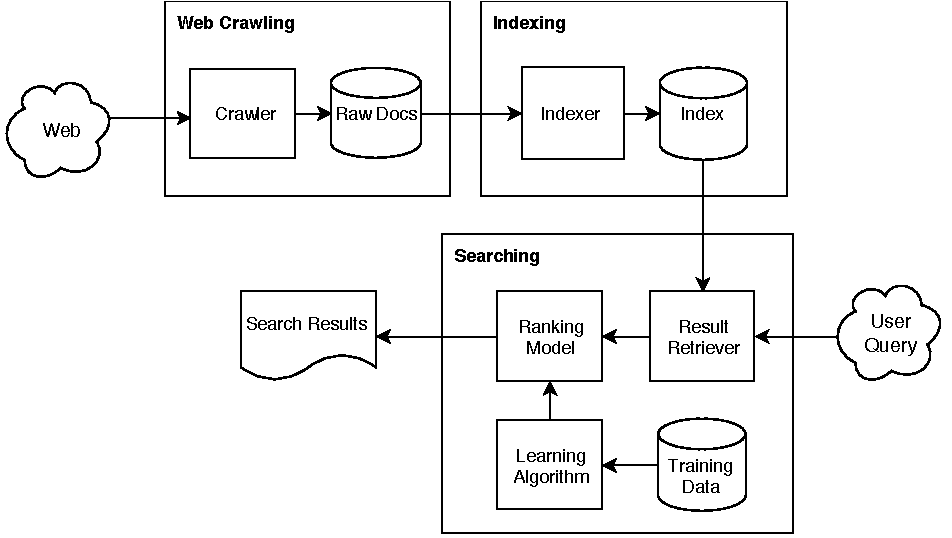
\includegraphics[width=0.8\textwidth]{img/searchengine.pdf}
  \caption{An example of a search engine architecture.}
  \label{fig:searchengine}
\end{figure}

Modern search engines use learning-to-rank algorithms for the ranking task. Learning to rank is the application of machine learning in information retrieval systems in order to construct ranking models. Such a model, typically supervised, is trained on training data consisting of query-document pairs, each with a relevance degree. The purpose of the model is to rank documents, i.e., produce an ordering that is optimal with respect to an evaluation metric.

Some of the evaluation metrics for ranking are mean average precision (MAP), discounted cumulative gain (DCG) and NDCG (normalized DCG), precision@n, NDCG@n (where @n denotes that the metrics are evaluated only on top n documents), mean reciprocal rank, Kendall's tau, and Spearman's rho. We use NDCG@n, so we will explain it in detail here. NDCG is a normalized version of discounted cumulative gain \citep{jarvelin2002cumulated}. Using a graded relevance scale of documents in a search-engine result set, DCG measures the usefulness, or gain, of a document based on its position in the result list. The gain is accumulated from the top of the result list to the bottom, with the gain of each result discounted at lower ranks. The graded relevance value is reduced logarithmically proportional to the position of the result, therefore penalizing highly relevant documents appearing lower in a search result list. The DCG at rank position $p$ is defined as:
\[ \mathrm {DCG_{p}} =\sum _{i=1}^{p}{\frac {rel_{i}}{\log _{2}(i+1)}}, \]
where $rel_{i}$ is the graded relevance of the result at position $i$.

We use normalized DCG, because search result lists vary in length depending on the query. In this case, the cumulative gain at each position for a chosen value of $p$ should be normalized across queries. We do this by sorting all relevant documents in the corpus by their relative relevance, producing the maximum possible DCG through position $p$, called Ideal DCG (IDCG) through that position. NDCG is defined as:
\[ \mathrm {nDCG_{p}} = \frac {\mathrm {DCG_{p}}}{\mathrm {IDCG_{p}}}, \]
and IDCG is defined as:
\[ \mathrm {IDCG_{p}} =\sum _{i=1}^{|REL|}{\frac {rel_{i}}{\log _{2}(i+1)}}, \]
where $|REL|$ represents the list of ordered relevant documents up to position $p$.

In an online scenario, when a user types a query into a search engine, they expect to see results in a very short time, typically a few hundred milliseconds. This makes it impossible to evaluate a complex ranking model, so modern search engines use a two-phase retrieval and ranking strategy \citep{cambazoglu2010early}. In the first phase, the scoring is very simple, enabling a quick retrieval process. Consequently, the second phase uses a more complex model, since now only a small subset of the overall document index is being ranked.

The query-document pairs are scored, then ranked, based on their feature vectors. The features can be divided into three groups:
\begin{enumerate}
	\item Query-independent or static features: features depending only on the document, but not on the query. For example, PageRank \citep{page1999pagerank} or the document's length. These features can be precomputed offline when indexing the document.
	\item Query-dependent or dynamic features: features depending both on the contents of the document and the query, such as the similarity between the query terms and the document content.
    \item Query features: features depending only on the query, such as the number of words in a query.
\end{enumerate}

\section{Problem Definition}
% talk about relevance vs recency and why it's difficult
The effectiveness of a search engine depends on the relevance of the result set it returns. Search engines employ ranking methods to provide the best results first. As more and more content is put on the Web, now more quickly than ever, the temporal aspect of results is very important for modern search engines. In web search, recency ranking refers to ranking the documents both by their relevance to the user query, and their freshness. The search engine can appear stale if it failed to recognize the temporal aspect of a query, which can also negatively affect the user experience. Effectively combining temporal features, as well as relevance-sensitive features in a ranking framework is still an open question for the research community.

The connection between relevance and recency is not always clear. In other words, if optimizing for only one of them, we might decrease the effectiveness of the search engine. Therefore, it is necessary to find an equilibrium. The trade-off can also depend on the user's query. For example, for a recency sensitive query, i.e., a query for which a user expects topically relevant documents to be also fresh, recency is very important. On the other hand, for timely queries, i.e., queries that do not show a spike in their popularity over time, relevance should be more important. Figure \ref{fig:serp} shows an example of a blend of relevant and recent results.

Even when the query type is identified, in order to incorporate both recent and relevant results, we need to determine the recency component on the document side. When dealing with general documents from the Web, this is not a trivial task, as most of the documents do not have any temporal information.

\begin{figure}
  \centering
  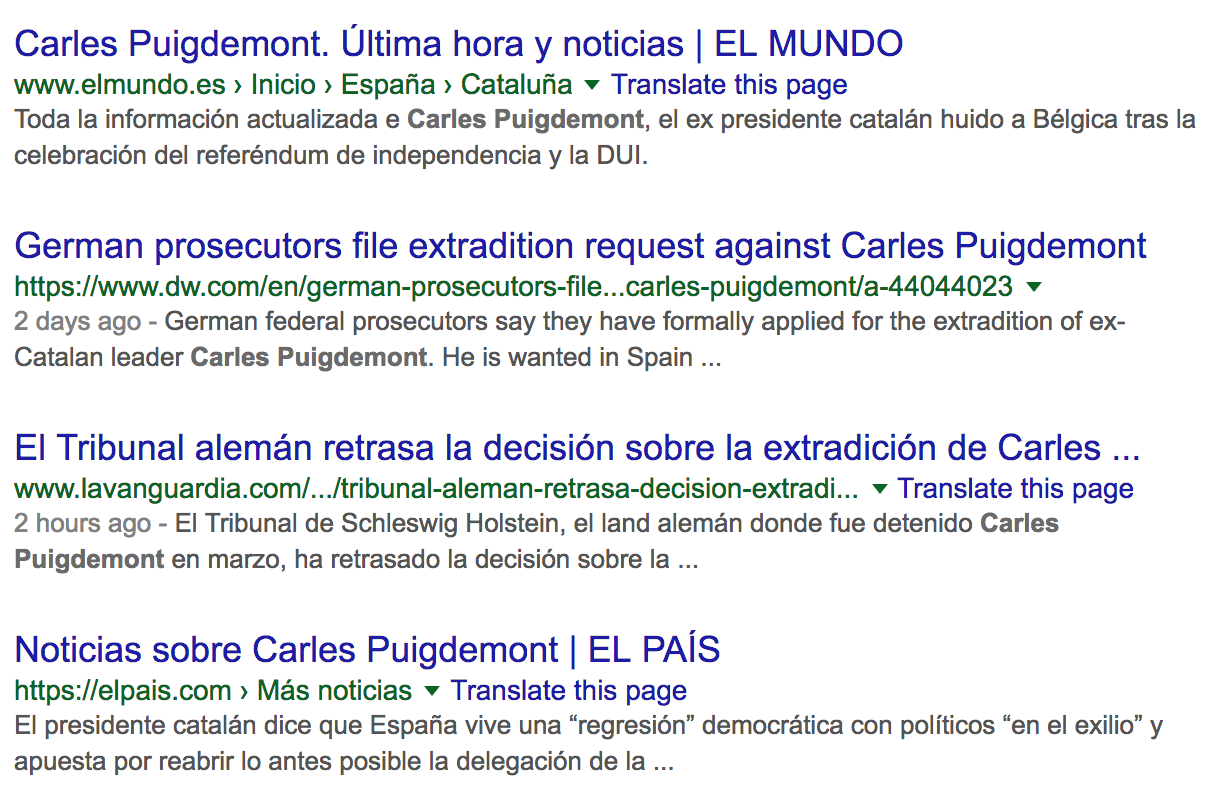
\includegraphics[width=0.7\textwidth]{img/serp.png}
  \caption{An example of a search engine result page (SERP) from Google for the query \textit{Carles Puigdemont} submitted on June 29, 2018.}
  \label{fig:serp}
\end{figure}

In our experiments, we ask the following research questions:
\begin{enumerate}
    \item How can we determine if a document's content is recent without having information on its publication date?
    \item How can we determine when queries seek recent results?
    \item How can we introduce recency ranking into an existing relevance ranking architecture?
\end{enumerate}

\section{Contributions}
The contributions of this thesis are both theoretical and practical. In Chapter~\ref{ch:doc}, we present a document age prediction model, used to predict how recent a document is by extracting temporal evidence from its content. In Chapter \ref{ch:query}, we present a query recency sensitivity classifier, used to predict the need of recent results for a query. Finally, in Chapter \ref{ch:webranking}, we present a novel method of incorporating recency with the help of these two classifiers into an existing search engine. We also present an exhaustive evaluation of all presented models.


\chapter{Related Work}
\label{ch:relatedwork}

% Carbon Dating The Web: Estimating the Age of Web Resources: https://arxiv.org/pdf/1304.5213.pdf

% Predicting document creation times: https://dbs.ifi.uni-heidelberg.de/files/Team/aspitz/publications/Spitz_et_al_Predicting_Document_Creation_Times.pdf

In the past decade, there have been a number of papers approaching the problem of combining relevance and recency in ranking. Some of them deal with more specific domains than web search, such as mail search \citep{carmel2017promoting}, microblog retrieval \citep{efron2012query}, and news search \citep{dakka2012answering}. In the domain of mail search, a recency-only ranking is traditionally implemented. Even when time-ranked results are mixed with relevance-based results, as \cite{carmel2017promoting} report, showing duplicate results to the user is not discouraged. These two key points make mail search a different problem than web search. Moreover, when it comes to news search, it is assumed that the publication date of the document is available \citep{dakka2012answering}. For the majority of documents on the Web, this is not the case, making web search a more difficult problem.

The works that directly improve ranking recency in web search are \citep{dong2010towards,dong2010time,dai2011learning,styskin2011recency}. \citet{dong2010towards} focus on breaking-news queries and build different rankers. If a query is classified as recency-sensitive, a recency-sensitive ranker is used to rank the documents matching that query. Similar to our work, they model different time slots by building language models from different sources (news content and queries) and compare them in order to classify if a query is recency-sensitive or not. Furthermore, they extract recency features from documents, and define the \textit{page age} as the time between the query submission time and page publication time, which is either the page creation time or the time it was last updated. The recency features they extract from documents are content-based and link-based. In our approach, we only extract content-based evidence. Finally, they manually annotate query-url pairs and train two separate models: a recency ranker and a relevance ranker. The key difference between this work and ours is that we do not manually annotate data, but automatically produce labels, we use only one ranking model for all queries, and we focus on all types of queries.

Extending their existing approach, \citet{dong2010time} introduce Twitter features to help with recency ranking. However, they do not focus on the fresh content produced by tweets to determine if the query terms are recency-sensitive, but instead they employ a URL mining approach to detect fresh URLs from tweets and learn to rank them.

Instead of having separate rankers, \citet{dai2011learning} propose a machine learning framework for simultaneously optimizing recency and relevance, focusing on improving the ranking of results for queries based on their temporal profiles. They determine the temporal profile of a query by building a time series of the relevant documents' content changes. Next, they extract temporal features from the seasonal-trend decomposition of different time series. We could not use this approach, as we only keep the most updated snapshot of documents in our index.

Similarly, \citet{cheng2013fresh} model term distribution of results over time and conclude that this change is strongly correlated with the users' perception of time sensitivity. However, they only focus on improving ranking for timely queries, i.e., queries that have no major spikes in volume over time, but still favour more recently published documents. In a similar work, \citet{efron2011estimation} assume that the document publication time is known. They compute a query-specific parameter that captures recency-sensitivity and is calculated based on the distribution of the publication times of the top retrieved documents by a relevance-based ranker.

However, when document publication time is not known, we have to search for other indicators of document recency and query recency sensitivity. For example, \citet{campos2016gte} use temporal expressions from web snippets related to the query to improve the ranking. In this work, we do the same. Other possible sources of temporal features include click logs and query logs. \citet{wang2012joint} learn the relevance and recency models separately from two different sets of features. Their divide-and-conquer learning approach is similar to \citep{dai2011learning}, but in this work, they omit manually annotating data, and instead automatically infer labels using clickthrough data. We do not use click logs, but we do extract frequency features from our query log, similarly to \citep{metzler2009improving, lefortier2014online}.

So far, we have explained how related work has extended existing learning-to-rank algorithms to take into account both relevance and recency. Another approach to recency ranking is an aggregated search strategy. In other words, recent results are extracted from a fresh vertical (such as news articles) and subsequently integrated into the result page. The blending of results from different verticals is called result set diversification. Examples of this approach are \citep{lefortier2014online,styskin2011recency}. In these two papers, a classifier is used to score the recency sensitivity of a user query, and this score is used to determine to what extent the documents from the fresh vertical should be inserted. Even though we do not perform result set diversification, we share similarities with these papers. The query fresh intent detector from \citep{lefortier2014online} is similar to our query recency classifier in terms of features used, and we have modeled our query ground truth labels according to the distribution reported in \citep{styskin2011recency}.

\chapter{Document Age Prediction Model}
\label{ch:doc}

\definecolor{eclipseStrings}{RGB}{42,0.0,255}
\definecolor{eclipseKeywords}{RGB}{127,0,85}
\colorlet{numb}{magenta!60!black}
\colorlet{punct}{red!60!black}
\definecolor{delim}{RGB}{20,105,176}

\lstset{
  basicstyle=\ttfamily,
  columns=fullflexible,
  showstringspaces=false,
  commentstyle=\color{gray}\upshape,
  breaklines=true
}
\lstdefinelanguage{json}
{
%     morestring=[b]",
%     morestring=[d]'
  commentstyle=\color{eclipseStrings}, % style of comment
  stringstyle=\color{eclipseKeywords}, % style of strings
  numbers=left,
  frame=lines,
  %backgroundcolor=\color{gray}, %only if you like
  string=[s]{"}{"},
  comment=[l]{:\ "},
  morecomment=[l]{:"},
  literate=
  *{0}{{{\color{numb}0}}}{1}
  {1}{{{\color{numb}1}}}{1}
  {2}{{{\color{numb}2}}}{1}
  {3}{{{\color{numb}3}}}{1}
  {4}{{{\color{numb}4}}}{1}
  {5}{{{\color{numb}5}}}{1}
  {6}{{{\color{numb}6}}}{1}
  {7}{{{\color{numb}7}}}{1}
  {8}{{{\color{numb}8}}}{1}
  {9}{{{\color{numb}9}}}{1}
  {:}{{{\color{punct}{:}}}}{1}
  {,}{{{\color{punct}{,}}}}{1}
  {\{}{{{\color{delim}{\{}}}}{1}
  {\}}{{{\color{delim}{\}}}}}{1}
  {[}{{{\color{delim}{[}}}}{1}
  {]}{{{\color{delim}{]}}}}{1},
}

In order to model how recent a document is, we try to predict the time the current content was last updated. Given that information, we can define the document age as:
\[ documentAge = currentTime - documentLastUpdateTime \]
Here, $currentTime$ is the time when we are observing the document, for example, at query issue time.

If we know the last update time of a document, it is trivial to calculate the document age on the fly. For example, in the case of news search, it is almost always the case that we are provided with a publication time and we can simply use it as a feature, as seen in \citep{dakka2012answering}. Moreover, \citet{spitz2018predicting} have shown that, for news articles, we can also take advantage of the citation network, or the inbound and outbound links in the articles.

However, as we are focusing on documents on the Web in general, we cannot assume that we have this information readily available. To this end, we developed a machine-learned model to predict the last update time of a document.

We approach this as a supervised regression problem, so we first obtain a labeled set of documents to serve as ground truth. We extract features from the content of the document which indicate when the document was last updated, and learn and evaluate a machine learning model. We explain how we compile the ground truth in the next section.

\section{Ground Truth Creation}
We create a ground truth set for a random sample of 5K documents from our document index. Instead of manually annotating the time a document was last updated, we infer it automatically by querying the Memgator web service.\footnote{\url{http://memgator.cs.odu.edu/}.} As described by \citet{salaheldeen2013carbon}, this service can be used for navigating between the current and the past web. It provides a list of \textit{mementos}, or timestamps, when the document was changed. We note that a memento timestamp is the time of capture at the web archive, which might not entirely align with the actual update time of the document. However, we deemed this approximation good enough for our purposes.

For a given URI, the service returns a list of timestamps, ordered from oldest to newest, when there was an update to the Web page. Figure \ref{code:memgator} shows an example of a request and response from the service. The list of mementos is shortened for readability.

\begin{lstlisting}[language=json,firstnumber=1,caption=Example of a request to and response from the Memgator web service., label=code:memgator]]
curl "https://memgator.cs.odu.edu/timemap/json/www.ntent.com"
{
  original_uri: "http://www.ntent.com",
  self: "https://memgator.cs.odu.edu/timemap/json/www.ntent.com",
  mementos: {
    list: [
      {
        datetime: "2000-04-08T22:25:51Z",
        uri: "http://web.archive.org/web/20000408222551/www.ntent.com:80/"
      },
      (...)
      {
        datetime: "2018-06-14T23:55:54Z",
        uri: "http://web.archive.org/web/20180614235554/www.ntent.com/"
      }
  ]
    first: {
        datetime: "2000-04-08T22:25:51Z",
        uri: "http://web.archive.org/web/20000408222551/www.ntent.com:80/"
    },
    last: {
        datetime: "2018-06-14T23:55:54Z",
        uri: "http://web.archive.org/web/20180614235554/www.ntent.com/"
    }
  }
\end{lstlisting}

A naïve approach would be to take the \texttt{last} field from the JSON, signifying the time of the last recorded change. However, when dealing with documents on the Web, it is often the case that an update is not actually a content update, but a page maintenance update. In other words, the change in document content is negligible and we do not want to capture such \textit{near-duplicates}.

To make sure we are capturing actual content updates, we traverse the list of last updates in reverse, from the latest to oldest timestamp, and compare the current document content to the previous one. If the similarity is above a certain threshold ($t$ = 90\%), we discard the update and keep going back in time. We compute the similarity between two documents by \textit{shingling} them \citep{broder1997resemblance}.

Shingling is a technique used in information retrieval to detect near-duplicate documents. Given a positive integer $k$ and a sequence of terms in a document $d$, we define the $k$-shingles of $d$ to be the set of all consecutive sequences of $k$ terms in $d$. Let $S(d_j)$ denote the set of shingles of document $d_j$. For example, for $d$ = \textit{Barcelona is the capital of Catalonia}, and $k = 3$, the shingles are \{(Barcelona, is, the), (is, the, capital), (the, capital, of), (capital, of, Catalonia)\}. We then produce an MD5 hash of each shingle, sort them alphabetically, and take the first $N$ shingles as a set. We denote this as $S(d_j)$. We compute the Jaccard coefficient to measure the degree of overlap between the sets $S(d_1)$ and $S(d_2)$ as:
\[ J(S(d_1),S(d_2)) = \frac{\vert S(d_1) \cap S(d_2)\vert}{\vert S(d_1) \cup S(d_2)\vert}. \]

\noindent If $J(S(d_1),S(d_2)) < 0.90$, the documents are assumed to be distinct.

Finally, the ground truth dataset consists of $5248$ documents, where each document object contains the following fields:
\begin{enumerate}
	\item \texttt{URL.} The full URL of a document, also a unique identifier of a document.
	\item \texttt{FullHTML.} The full HTML content retrieved by the crawler, without any preprocessing.
    \item \texttt{ContentHTML.} The content of the document after boilerplate removal was performed. This does not contain JavaScript blocks, CSS, and such.
    \item \texttt{DocumentLastUpdateTime.} The target variable, obtained using the aforementioned technique, expressed as Unix time.\footnote{Unix time is the number of seconds that have elapsed since January 1, 1970.}
\end{enumerate}

\section{Feature Extraction}
We extract features from the URL and the content of the document. For the content, we process both the full HTML of the document (before boilerplate removal), and from the clean HTML (after boilerplate removal). Table \ref{tb:dataset-doc} shows the statistics of the documents from our ground truth. The average length of the raw document HTML is ten times longer than the clean one. Although some of this is due to the HTML format (e.g., tags and attributes), there is still a lot of noisy content that could be used to extract features indicative of the document's last modification date. Therefore, we choose to process both versions of the document, and have both groups of extracted features in the resulting feature vector.

\begin{table}[h!]
\centering
\caption{Ground truth dataset statistics.}
\label{tb:dataset-doc}
\begin{tabular}{@{}cccc@{}}
\toprule
Number of documents & Average FullHTML size & Average ContentHTML size &  \\ \midrule
5248 & 108054 characters & 10961 characters &  \\ \bottomrule
\end{tabular}
\end{table}

First, we develop a pattern-matching solution to extract any mention of dates. A comprehensive list of supported date formats is shown in Table \ref{tb:dates}.

\begin{table}[!htbp]
\centering
\caption{Date formats supported in regular expressions.}
\label{tb:dates}
\begin{tabular}{@{}ll|ll@{}}
\toprule
Date format & Example date & Date format & Example date \\ \midrule
dd/mm/yy & 27/05/93 & yy-mmm-dd & 93-Aug-27 \\
dd/mm/yyyy & 27/05/1993 & yy-mmmm-dd & 93-August-27 \\
d/m/yy & 5/5/93 & mm/dd/yy & 05/27/93 \\
d/m/yyyy & 5/5/1993 & mm/dd/yyyy & 05/27/1993 \\
dd-mmm-yy & 27-Aug-93 & mmm-dd-yy & Aug-27-93 \\
dd-mmm-yyyy & 27-Aug-1993 & mmm-dd-yyyy & Aug-27-1993 \\
d-mmmm-yy & 27-August-93 & mmmm dd, yyyy & August 27, 1993 \\
d-mmmm-yyyy & 27-August-1993 & dd mmmm yyyy & 27 August 1993 \\
yy/mm/dd & 93/05/27 & mmm yyyy & Aug 1993 \\
yyyy/mm/dd & 1993/05/27 & mmmm, yyyy & August, 1993 \\
yyyy-mm-dd & 1993-05-27 & yyyy & 1993 \\ \bottomrule
\end{tabular}
\end{table}

We denote the features that capture dates as \texttt{timestamp features}. When extracting timestamps containing uncertainty of the exact date, we take the approach as \citet{berberich2010language}. More specifically, we support both Americanized date formats (first month, then day) and standardized (first day, then month). We use several regular expressions to capture different date formats, transform all dates to a standardized format \texttt{YYYY-MM-DD}, then convert the extracted dates to Unix time. Moreover, since we aim to predict the last update time on a year-month scale, we set the day field to the 15th of the month.

Apart from the \texttt{timestamp features}, we also extract features from specific \texttt{<meta>} tags, called \texttt{meta tag features}, and the \texttt{jQuery version feature}. The total number of features is 20, where each feature value is expressed as Unix time. The list of features is shown in Table \ref{tb:features}.

\begin{table}[]
\centering
\caption{List of features.}
\label{tb:features}
\begin{tabular}{@{}cl@{}}
\toprule
Feature index & Feature name                                     \\ \midrule
1             & TimestampFeatures\_FullHtml\_MinTimestamp        \\
2             & TimestampFeatures\_FullHtml\_MaxTimestamp        \\
3             & TimestampFeatures\_FullHtml\_AvgTimestamp        \\
4             & TimestampFeatures\_FullHtml\_FirstTimestamp      \\
5             & TimestampFeatures\_FullHtml\_LastTimestamp       \\
6             & TimestampFeatures\_FullHtml\_MostCommonYear      \\
7             & TimestampFeatures\_FullHtml\_MostCommonYearMonth \\
8             & TimestampFeatures\_Html\_MinTimestamp            \\
9             & TimestampFeatures\_Html\_MaxTimestamp            \\
10            & TimestampFeatures\_Html\_AvgTimestamp            \\
11            & TimestampFeatures\_Html\_FirstTimestamp          \\
12            & TimestampFeatures\_Html\_LastTimestamp           \\
13            & TimestampFeatures\_Html\_MostCommonYear          \\
14            & TimestampFeatures\_Html\_MostCommonYearMonth     \\
15            & MetaTagFeatures\_FullHtml\_LastModified                   \\
16            & MetaTagFeatures\_FullHtml\_Copyright                      \\
17            & MetaTagFeatures\_FullHtml\_DCDateIssued                   \\
18            & MetaTagFeatures\_FullHtml\_DCTermsModified                \\
19            & JQueryVersion                                    \\
20            & TimestampFeatures\_Url                                     \\ \bottomrule
\end{tabular}
\end{table}

\subsection{Timestamp Features}
We extract \texttt{timestamp features} from the full HTML of the document (pre-boilerplate removal), the clean HTML (post-boilerplate removal), and document URL. We want to be able to predict the last update time of a document on a monthly scale, so we only store the year and month of retrieved timestamps, whereas we always set the day value to the 15th.

The \texttt{timestamp features} are the following:
\begin{itemize}
	\item \texttt{MinTimestamp:} the minimal timestamp mentioned;
    \item \texttt{MaxTimestamp:} the maximal timestamp mentioned;
    \item \texttt{AvgTimestamp:} the average timestamp mentioned;
    \item \texttt{FirstTimestamp:} the first timestamp mentioned;
    \item \texttt{LastTimestamp:} the last timestamp mentioned;
    \item \texttt{MostCommonYear:} the most commonly mentioned year, converted to June 15th of that year;
    \item \texttt{MostCommonYearMonth:} the most commonly mentioned year and month, converted to the 15th of that month.
\end{itemize}

We also extract any timestamps that are mentioned in the URL and model it as a separate feature.

\subsection{Other Features}
For the \texttt{meta tag features}, we capture four different tag types:

\begin{lstlisting}[language=json]
<meta name="Last-Modified" content="2017-06-05 11:21:43">
<meta name="copyright" content="Copyright (c) 2017 ABC News Internet Ventures">
<meta name="dcterms.modified" content="2007-12-20 11:17:23">
<meta property="DC.date.issued" content="2017-04-27T08:00:40-04:00">
\end{lstlisting}

Lastly, for the \texttt{jQuery feature}, we precomputed a lookup table of release dates of different jQuery versions.\footnote{\url{https://gist.github.com/0xdevalias/8e558f4ed452ec54880e8b8445d13e28 }.} Often times, documents include a snippet referencing the minimum jQuery version, such as:
\begin{lstlisting}[language=json]
<script src="https://ajax.googleapis.com/ajax/libs/jquery/1.7.2/jquery.min.js"></script>
\end{lstlisting}

If there is a mention of a jQuery version number in the full HTML, we set the \texttt{jQuery feature} value as the release date of that version.

\section{Model Training}
% what is a train instance, framework used, feature importance
We use Gradient Boosted Regression Trees (GBRT) as the model. Gradient boosting is a machine learning technique where the prediction model is an ensemble of weak prediction models, in this case decision trees. The idea of gradient boosting was first introduced by \citet{breiman1997arcing}. Later, \citet{friedman2001greedy} introduced improvements to the boosting algorithms.

Decision trees were suitable for this problem, as they are easy to interpret, they require little data preparation, and have built-in feature selection. We use XGBoost (eXtreme Gradient Boosting), introduced by \citet{chen2016xgboost}, an open-source parallel gradient boosting library to train and evaluate the model.

As mentioned earlier, we have a total of 20 features, where each feature value is Unix time. Each training instance is of the \texttt{LibSVM data format}:\footnote{\url{https://www.csie.ntu.edu.tw/~cjlin/libsvm/}.}
\[ \texttt{<label> <index\_1>:<value\_1> ... <index\_N>:<value\_N>} \]

Here, \texttt{<label>} is the target value, expressed in Unix time, and the rest of the fields model the feature index and value, respectively.

To investigate which features are more useful than others, we plot the feature importance scores, as seen in Figure \ref{fig:fscores}. By looking at the feature overview in Table \ref{tb:features}, we can see that the first five features, \texttt{timestamp features} retrieved from the full HTML content, are the most important, followed by \texttt{timestamp features} retrieved from the clean HTML. The worst-performing group of features are the \texttt{meta tag features}, due to the fact that these attributes are seldom included in documents in our collection. The same applies for the \texttt{jQuery version feature}, which, although very indicative of the document publication date, was rarely present in our document set.

\begin{figure}
  \centering
  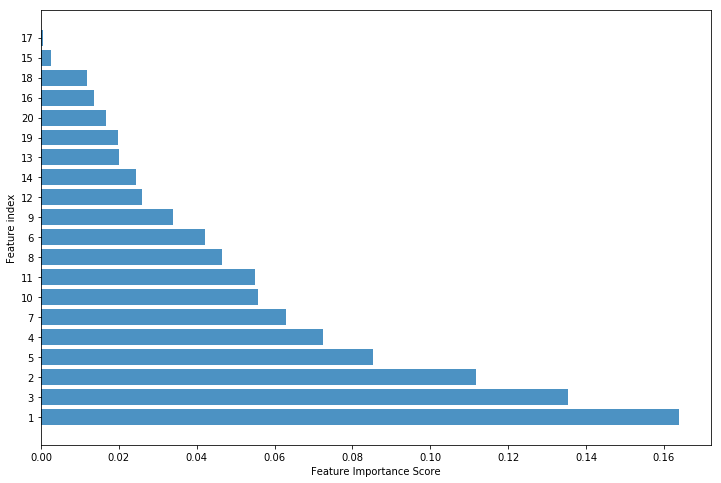
\includegraphics[width=\linewidth]{img/doc_f_importance.png}
  \caption{Feature importance scores of the document age prediction model.}
  \label{fig:fscores}
\end{figure}
% plotted in queries.ipynb

% add/expand discussion of features, how often they're present, why we chose them etc.

\section{Evaluation}
\label{sec:docparams}
For training the model, we split the input set into train and validation sets in the 70:30 ratio. We then proceeded to grid search the hyper-parameters of the model using a 5-fold cross-validation. Listing~\ref{param-doc} shows which hyper-parameters are tuned.

\begin{lstlisting}[language=json,caption=Hyper-parameter tuning for the document age model.,label=param-doc]
'max_depth': [4, 6, 8, 10], (best = 4)
'min_child_weight': [0, 1, 2], (best = 0)
'gamma': [0.0, 0.1, 0.2, 0.3], (best = 0.0)
'subsample': [0.6, 0.8, 1.0], (best = 1.0)
'colsample_bytree': [0.6, 0.8, 1.0], (best = 0.6)
'learning_rate': [0.01, 0.03, 0.1, 0.2, 0.3], (best = 0.01)
'n_estimators': [100, 500, 1000, 5000],  (best = 1000)
\end{lstlisting}

%  Best hyperparameters:
% {'colsample_bytree': 0.6, 'learning_rate': 0.01, 'min_child_weight': 0, 'n_estimators': 1000, 'subsample': 1.0, 'max_depth': 4, 'gamma': 0.0}
% RMSE (train) 32026382.3785 or 3.202e+07
% RMSE (test): 3.596e+07

Parameter \texttt{max\_depth} is the maximum depth of a tree, and increasing this value will make the model more complex and likely to overfit. Parameter \texttt{min\_child\_weight} is the minimum sum of instance weight needed in a child to continue further partitioning. The larger, the more conservative the model. Parameter \texttt{gamma} is the minimum loss reduction required to make a further partition on a leaf node of the tree. The larger, the more conservative the model. Parameter \texttt{subsample} is the ratio of training instances to subsample. Setting it to 0.5 means that XGBoost randomly collects half of the data instances to grow trees and this will prevent overfitting. Parameter \texttt{colsample\_bytree} is the subsample ratio of columns when constructing each tree. Parameter \texttt{learning\_rate} is the step size shrinkage used in the update phase to prevent overfitting. Parameter \texttt{n\_estimators} is the number of trees to construct.

The training of the model took 23 hours on a machine with CentOS 7.5.1804, 16 GB of RAM, and 8 Intel(R) Xeon(R) CPU E5-2660 v3 @ 2.60GHz CPUs. The model was trained by minimizing the root mean squared error (RMSE) of the difference between the predicted Unix time value and the value from the ground truth. 

The results on the train and test sets are shown in Table \ref{tb:docclass}. To provide a better intuition for the results, the epoch timestamp (or Unix time) of \texttt{26 June 2018} is $1529971200$. Moreover, an RMSE value of $3e+07$ is equivalent to \texttt{14 December 1970}. Since Unix time is defined as the number of seconds since \texttt{1 January 1970}, we can conclude that the model's predictions are accurate within a year.

\begin{table}[h!]
\centering
\caption{Document age prediction model evaluation.}
\label{tb:docclass}
\begin{tabular}{@{}ll@{}}
\toprule
RMSE train & RMSE test \\ \midrule
3.202e+07  & 3.596e+07 \\ \bottomrule
\end{tabular}
\end{table}

To gain insight into how our model is performing, we plot two different learning curves. The first learning curve, shown in Figure \ref{fig:doc-curve1}, shows the model performance based on the number of training rounds. We run a 5-fold cross-validation on different subsets of training instances. We expect to see an increase in the error on the training set, as we increase the number of training instances. This is because the model is likely to overfit and predict well when given a smaller number of training instances. However, as the model is trained on more data, it manages to fit better the validation set. Thus, the validation error decreases. Based on this graph, it looks like we could benefit from adding more training instances, and still not be at risk of overfitting the model.

The second learning curve is shown in Figure \ref{fig:doc-curve2}. Here, we examine the model's performance based on the number of training rounds. We notice that both the training and validation error reduce rapidly. Nevertheless, the validation error does not reduce significantly after 400 rounds. If we wanted to reduce the time and computational power necessary to train the model, this graph shows we can stop training after 400 rounds, since no significant improvement is observed after that point. Note, however, that we trained the model with setting the configuration parameter \texttt{early\_stopping\_rounds} to 50, which means there was a reduction in validation error after all.

\begin{figure}
\centering
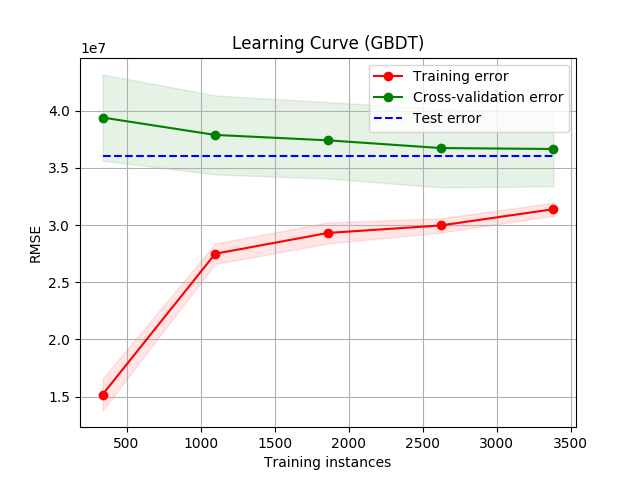
\includegraphics[width=0.8\linewidth]{img/doc_learning_curve.png}
\caption{Learning curve of the document age prediction model based on the number of training instances.}
\label{fig:doc-curve1}
\end{figure}

\begin{figure}
\centering
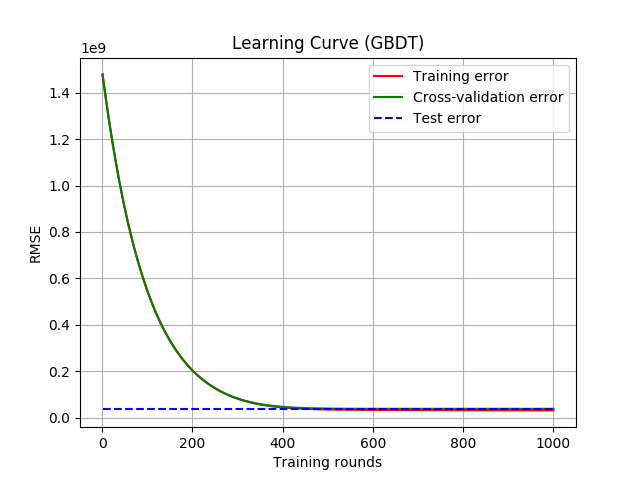
\includegraphics[width=0.8\linewidth]{img/doc_learning_curve2.png}
\caption{Learning curve of the document age prediction model based on the number of training rounds.}
\label{fig:doc-curve2}
\end{figure}



\chapter{Query Recency Sensitivity Model}
\label{ch:query}

\definecolor{eclipseStrings}{RGB}{42,0.0,255}
\definecolor{eclipseKeywords}{RGB}{127,0,85}
\colorlet{numb}{magenta!60!black}
\colorlet{punct}{red!60!black}
\definecolor{delim}{RGB}{20,105,176}

\lstset{
  basicstyle=\ttfamily,
  columns=fullflexible,
  showstringspaces=false,
  commentstyle=\color{gray}\upshape,
  breaklines=true
}
\lstdefinelanguage{bash}
{
%     morestring=[b]",
%     morestring=[d]'
  commentstyle=\color{eclipseStrings}, % style of comment
  stringstyle=\color{eclipseKeywords}, % style of strings
  numbers=left,
  frame=lines,
  %backgroundcolor=\color{gray}, %only if you like
  string=[s]{"}{"},
  comment=[l]{:\ "},
  morecomment=[l]{:"},
  moredelim=**[is][\color{blue}]{?}{?},
  moredelim=**[is][\color{orange}]{!}{!},
  moredelim=**[is][\color{red}]{^}{^}
}

A web search query is a query that a user enters into a web search engine to satisfy their information needs. As described by \citet{broder2002taxonomy}, queries have empirically been divided into three different groups:
\begin{itemize}
	\item Informational queries: queries that cover a broad topic for which there may be thousands of relevant results (e.g., \textit{barcelona}).
	\item Navigational queries: queries that seek a single website or web page of a single entity (e.g., \textit{youtube}, \textit{facebook}).
	\item Transactional queries: queries that reflect the intent of the user to perform a particular action, such as downloading a screen saver.
\end{itemize}

Another possible division of queries can be according to their temporal profiles, as defined by \citet{jones2007temporal}. They propose three temporal classes of queries:
\begin{itemize}
	\item Atemporal queries: queries that take place at any time.
    \item Temporally unambiguous queries: queries that take place at a specific period in time.
    \item Temporally ambiguous: queries that take place during one of several possible episodes.
\end{itemize}

\begin{figure}
\centering
\begin{subfigure}{.5\textwidth}
  \centering
  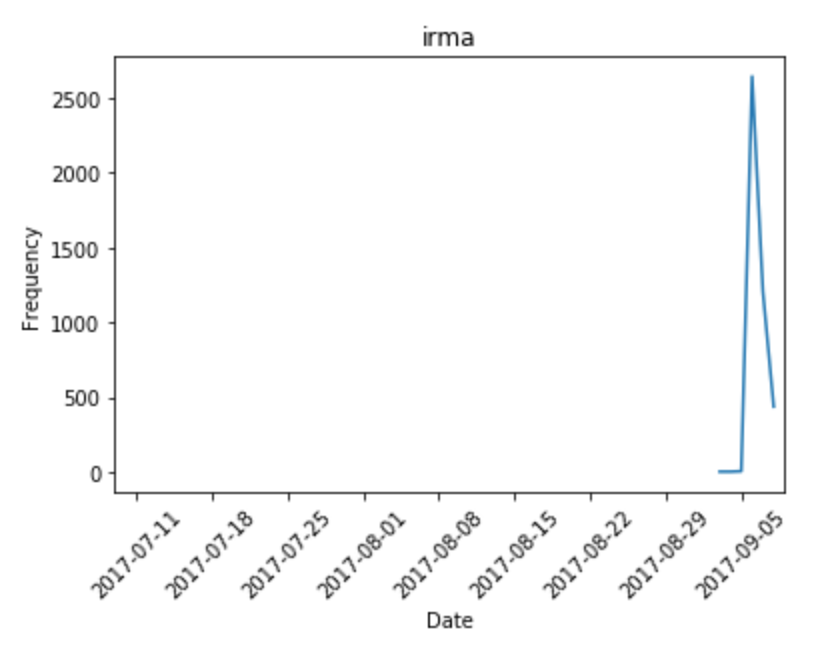
\includegraphics[width=.8\linewidth]{img/query1.png}
  \caption{A temporally unambiguous query.}
  \label{fig:query1}
\end{subfigure}%
\begin{subfigure}{.5\textwidth}
  \centering
  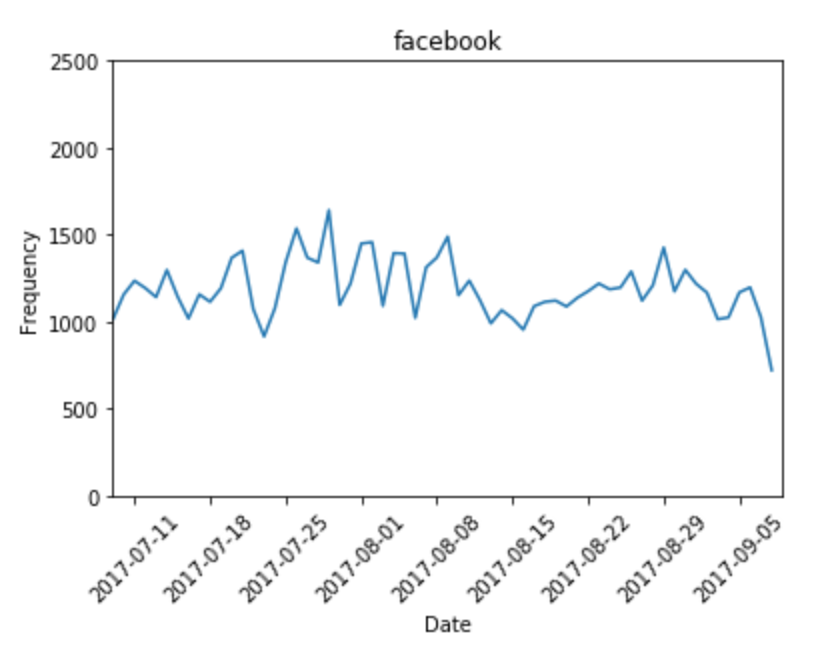
\includegraphics[width=.8\linewidth]{img/query2.png}
  \caption{An atemporal query.}
  \label{fig:query2}
\end{subfigure}
\caption{Examples of queries with different temporal profiles.}
\label{fig:query-temporal}
\end{figure}

Figure \ref{fig:query-temporal} shows an example of queries with different temporal profiles. The query \textit{irma} is temporally unambiguous, as it refers to the hurricane Irma, whereas the query \textit{facebook} is atemporal.

User experience is improved by integrating recency of retrieved results for most types of queries. Therefore, instead of focusing on a specific query type, we choose to introduce the recency vertical for queries in general.

As described by \cite{styskin2011recency}, not all queries require the same percentage of recent results, and not all queries seek the same granularity of result recency (e.g., hours, days, years). We call this property \textit{query recency sensitivity}. We argue that the inference of query's recency sensitivity has an impact on the ranking of retrieved results.

In a conventional information retrieval setting, a query instance is defined only as the query string. However, as we are introducing a recency component, we have to capture the temporal aspect of the query as well. For example, for the query \textit{stephen hawking}, the user might expect little to no change in results when submitting the same query in different points in time. Nonetheless, if searching for \textit{stephen hawking} on March 14, 2018, we would expect to see more breaking-news results than usually, since that was the day he died. Thus, in a query recency sensitivity setting, we define a query instance as:
\[ queryInstance = (queryText, submissionTime) \]

\noindent In other words, the same query can be submitted at different times, and yield a different ranking of results. \citet{styskin2011recency} also defined different levels of recency sensitivity. They define four labels of recency sensitivity and ask human judges to annotate real user queries. The labels are probabilities from $[0,1]$, and are defined as the following:
\begin{enumerate}
	\item \texttt{0.95}: the query is strictly about a recent event, e.g., \textit{stephen hawking death} on the day of the event;
    \item \texttt{0.75}: the query's primary interest is related to a recent event, but the user also wants just topically relevant results, e.g., \textit{oscar} on the day of the ceremony;
    \item \texttt{0.25}: the query’s primary interest is not likely to be focused on a particular event, but it makes sense to present some recent content, e.g., \textit{britney spears};
    \item \texttt{0}: otherwise, the query is assigned zero probability to be recency sensitive.
\end{enumerate}

\noindent We use these observations in constructing our ground truth dataset.

\section{Ground Truth Creation}
Instead of manually annotating queries, we choose to automatically infer recency sensitivity for queries. For this, we use a previously compiled ground truth dataset used for web ranking evaluation.\footnote{The details of this dataset cannot be disclosed, as it was constructed within a commercial project.} The dataset consists of $142807$ queries submitted to a third party search engine in the period of July 2017 -- September 2017.

Unfortunately, when this dataset was compiled, the query submission date was not recorded, as it was deemed unnecessary for relevance-based ranking evaluation. However, we were able to reconstruct it based on the order in which the queries were submitted, the rate they were submitted at, and the start and end date of the scraping. Since we are only able to reconstruct the submission date, not the exact time, we set the time as 23:59 of that day.

The queries were submitted to a third party search engine, and the first 50 results per query were scraped. An example of a partial result set for the query \textit{kardashian} is shown in Listing~\ref{serp}.

\begin{lstlisting}[language=json,firstnumber=1,caption=Example of retrieved results for a query., label=serp]]
{
  query_text: "kardashian",
  query_submission_date: "2017-08-27 23:59:00",
  results: {
    list: [
      {
        rank: "0",
        uri: "https://www.instagram.com/kimkardashian/?hl=en",
        title: "Kim Kardashian West (@kimkardashian): Instagram photos and videos",
        snippet: "103m Followers, 111 Following, 3933 Posts - See Instagram photos and videos from Kim Kardashian West (@kimkardashian)"
      },
      {
        rank: "1",
        uri: "https://en.wikipedia.org/wiki/Kim_Kardashian",
        title: "Kim Kardashian - Wikipedia",
        snippet: "Kimberly Kardashian West is an American reality television personality, socialite, actress, businesswoman and model. Kardashian first gained media attention..."
      },
      {
        rank: "2",
        uri: "http://people.com/babies/kanye-west-kim-kardashian-expecting-third-child-surrogate-pregnant/",
        title: "Kanye and Kim Kardashian West Expecting Third Child - People",
        snippet: "19 hours ago - Kim Kardashian and Kanye West Expecting Baby No. 3 via Surrogate! ..."
      },
      {
        rank: "3",
        uri: "http://people.com/babies/kim-kardashian-first-red-carpet-appearance-baby-number-3/",
        title: "Kim Kardashian Makes First Red Carpet Appearance Following News ...",
        snippet: "10 hours ago - Kim Kardashian West made her first red carpet appearance at New York Fashion Week on Wednesday following the news that she is expecting..."
      }
      (...)
    ]
  }
}
\end{lstlisting}

The snippet field shows the beginning of the document, and sometimes it includes information on when the document was published. This timestamp is relative to the query submission date, and can be in the form of \texttt{1-23 hours ago}, \texttt{2-7 days ago}, or a specific date, i.e., \texttt{May 27, 2018}. We take advantage of this temporal information when automatically determining which queries are more recency sensitive than others.

Our idea is to sort the queries in descending order based on a custom recency sensitivity function, then apply labels based on the distribution of the classes shown in Figure \ref{fig:query_dis}, and defined by \citet{styskin2011recency}. To score a query, we first take all the results with snippets that contain \texttt{1-23 hours ago}. We convert the relative timestamp to an absolute one by subtracting its value from the query submission time and express it as Unix time. We define the query score as the sum of the timestamps from the described snippets. Lastly, we sort the queries according to this score in descending order, and assign the label \texttt{0.95} to the first 0.73\% of queries, \texttt{0.75} to the next 1.11\%, \texttt{0.25} to the next 4.9\%, and \texttt{0.0} to the rest. Next, we downsample our query set from the initial $142807$ queries to $4000$ by maintaining the distribution of classes. Finally, we use this as ground truth for the query recency sensitivity model.

\begin{figure}
  \centering
  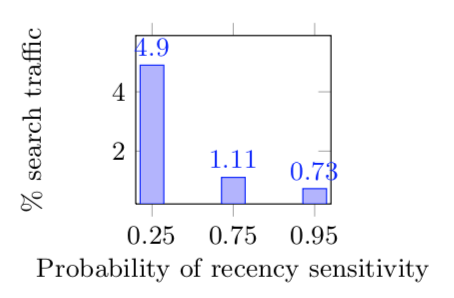
\includegraphics[width=0.4\textwidth]{img/query_distribution.png}
  \caption{Distribution of query recency sensitivity classes defined by \citet{styskin2011recency}.}
  \label{fig:query_dis}
\end{figure}

\section{Feature Extraction}

We use 34 features in our model. We extract features from three different sources:
\begin{itemize}
	\item Our query log. Features such as the number of times the query was submitted over different time periods, and the ratio of the number of submissions of the query in the last day and in the last week. Additionally, the probabilities of the query being generated by language models based on the query log over different time periods.
    \item The query itself. These are features such as the number of tokens, and several boolean features.
    \item Twitter. We mine recent tweets with respect to the query submission time, and generate language models based on tweets in the last day, week, and two weeks.
\end{itemize}

A comprehensive list of features can be seen in Table~\ref{tb:features-query}. Here, the first six features are extracted from the query log, the next four features from the query itself, and the rest of the features are probabilities of the query being generated by different language models. Language models built on tweets and using bigrams are denoted as \texttt{LM\_Tweet\_2}, and the ones using trigrams are \texttt{LM\_Tweet\_3}. The same applies for language models built on the query log, denoted as \texttt{LM\_QL}.

\begin{table}[]
\centering
\caption{List of features.}
\label{tb:features-query}
\begin{tabular}{@{}cl@{}}
\toprule
Feature index & Feature name \\ \midrule
1 & QuerySubmissions\_LastDay \\
2 & QuerySubmissions\_LastWeek \\
3 & QuerySubmissions\_LastMonth \\
4 & QuerySubmissions\_Day/Week \\
5 & QuerySubmissions\_Day/Month \\
6 & QuerySubmissions\_Week/Month \\
7 & Contains\_News \\
8 & Contains\_Now \\
9 & Contains\_Numeral \\
10 & NumberTokens \\
11 & LM\_Tweet\_2\_Day \\
12 & LM\_Tweet\_2\_Week \\
13 & LM\_Tweet\_2\_TwoWeeks \\
14 & LM\_Tweet\_2\_Day/Week \\
15 & LM\_Tweet\_2\_Day/TwoWeeks \\
16 & LM\_Tweet\_2\_Week/TwoWeeks \\
17 & LM\_Tweet\_3\_Day \\
18 & LM\_Tweet\_3\_Week \\
19 & LM\_Tweet\_3\_TwoWeeks \\
20 & LM\_Tweet\_3\_Day/Week \\
21 & LM\_Tweet\_3\_Day/TwoWeeks \\
22 & LM\_Tweet\_3\_Week/TwoWeeks \\
23 & LM\_QL\_2\_Day \\
24 & LM\_QL\_2\_Week \\
25 & LM\_QL\_2\_Month \\
26 & LM\_QL\_2\_Day/Week \\
27 & LM\_QL\_2\_Day/Month \\
28 & LM\_QL\_2\_Week/Month \\
29 & LM\_QL\_3\_Day \\
30 & LM\_QL\_3\_Week \\
31 & LM\_QL\_3\_Month \\
32 & LM\_QL\_3\_Day/Week \\
33 & LM\_QL\_3\_Day/Month \\
34 & LM\_QL\_3\_Week/Month \\ \bottomrule
\end{tabular}
\end{table}

\subsection{Language Model Features}

Language models are models that assign probabilities to sequences of words, or in our case, queries. We use language models to determine the probability of a query being generated by a set of tweets or queries in our query log over different time periods.

Formally, an $n$-gram language model makes the assumption that the probability of a word only depends on the previous $n$ words. Therefore, the probability $P(w_{1},\ldots ,w_{m})$ of observing the sentence $w_{1},\ldots ,w_{m}$ is approximated as:
\[ P(w_{1},\ldots ,w_{m})=\prod _{{i=1}}^{m}P(w_{i}\mid w_{1},\ldots ,w_{{i-1}})\approx \prod _{{i=1}}^{m}P(w_{i}\mid w_{{i-(n-1)}},\ldots ,w_{{i-1}}) \]

\noindent The conditional probability can be calculated from $n$-gram model frequency counts:
\[ P(w_{i}\mid w_{{i-(n-1)}},\ldots ,w_{{i-1}})={\frac  {{\mathrm  {count}}(w_{{i-(n-1)}},\ldots ,w_{{i-1}},w_{i})}{{\mathrm  {count}}(w_{{i-(n-1)}},\ldots ,w_{{i-1}})}} \]

A common problem when using frequency counts directly is the sparsity of the data. In other words, many words will yield zero and the overall probability will be zero. To prevent this, a technique called \textit{smoothing} is used to assign some probability to unseen words. Various techniques exist, the simplest one being \textit{add-one smoothing}, or assigning a count of 1 to unseen words. The most commonly used technique is the interpolated Kneser-Ney algorithm \citep{kneser1995improved}.

We use the KenLM Language Model Toolkit\footnote{\url{https://kheafield.com/code/kenlm/}.} to construct our language models. The toolkit uses linear probing for storing the frequency counts and the Kneser-Ney algorithm for smoothing. The toolkit is decribed in detail in \citep{Heafield-kenlm} and \citep{Heafield-estimate}. The usage is straightforward and consists of two steps: estimating (building) the language models, and querying them (producing probabilities for queries).

An example for a bigram language model is shown in Listing \ref{kenlm}. First, we estimate a language model by providing a corpus (in our case either tweets or queries in our query log), and the order of the model (in this case, two for bigrams). Next, we convert the produced ARPA file to a binary format to reduce loading time. Finally, we query the model by providing the queries as input, and get probabilities of the queries being generated by that language model as the output.

\begin{lstlisting}[language=bash,firstnumber=1,caption=Estimating a bigram language model and producing predictions for queries., label=kenlm]]
?kenlm/bin/lmplz? !-o! 2 < INPUT_CORPUS > model.2.arpa
?kenlm/bin/build_binary? model.2.arpa model.2.binary
?kenlm/query? !-v! sentence model.2.arpa < INPUT_QUERIES > OUTPUT_PROBABILITIES
\end{lstlisting}

\subsubsection{Query log corpus}
We estimate language models based on our query log by first extracting the corresponding corpus. For a date $d$, we create language models based on the queries in our query log from the previous day, week, and month. As explained earlier, our ground truth consists of queries submitted in the period of July 2017 -- September 2017. For each date $d$ from this time period, we model three different time slots $t$, and two different types of language models, bigrams and trigrams, which amounts to six language models per date $d$.

Inspired by \citet{dong2010towards}, our idea is to compare the probabilities for the input query to be generated by language models $LM_{Q,t}$, where $t \in \{\text{prev\_day}, \text{prev\_week}, \\ \text{prev\_month}\}$. If there is a spike in interest for a given query, resulting in more traffic and, consequently, higher need for recent results, we expect the probability of $LM_{Q,{\rm prev\_day}}$ to be higher than $LM_{Q, {\rm prev\_week}}$ and especially $LM_{Q, {\rm prev\_month}}$. Features with indices 23--34 in Table \ref{tb:features-query} model the probabilities of different $LM_{Q,t}$, as well as their ratios.

\subsubsection{Twitter corpus}
Similar to the query log corpus, our idea is to extract a corpus of tweets from different time slots, construct language models, and model the probabilities for the input query to be generated by these language models. In this case, we build language models $LM_{T,t}$, where $t \in \{\text{prev\_day}, \text{prev\_week}, \text{prev\_two\_weeks}\}$. Features with indices 11--22 in Table \ref{tb:features-query} model the probabilities of different $LM_{T,t}$, as well as their ratios.

For the queries in our ground truth, collecting the tweets is simple since we are able to do it in an offline manner. More specifically, we download a precompiled archive of tweets produced by The Internet Archive,\footnote{\url{https://archive.org/about/}.} a nonprofit digital library. They provide monthly archives of tweets, sampled from the general Twitter stream, as a simple collection of JSON objects.

In an online setting, where we cannot download a precompiled archive, we use a Python library called \texttt{twarc}\footnote{\url{https://github.com/docnow/twarc}.} to grab fresh tweets. The library queries the Twitter API, handles Twitter API's rate limits, and stores the retrieved tweets as JSON objects. Before querying the API, we register our developer application with Twitter to use the Standard search API,\footnote{\url{https://developer.twitter.com/en/docs/tweets/search/api-reference/get-search-tweets}.} which means we are able to retrieve only the past seven days of tweets. 

We contributed to this library by adding the parameter \texttt{until}, which is a date specifying the cut-off date for tweet creation date. This option was needed because \texttt{twarc} downloads tweets for a specific date until exhaustion, which takes too long, so we decide to run the tweet retrieval separately for each day in the past week. Moreover, the library does not support stopping after retrieving a certain number of tweets, so we used the \texttt{timeout.sh} script written by Anthony Thyssen\footnote{\url{http://www.ict.griffith.edu.au/anthony/software/#timeout}.} to terminate the process after a certain time elapsed. An example of collecting tweets from a specific date is shown in Listing \ref{twarc}.

\begin{lstlisting}[language=bash,firstnumber=1,caption=Downloading a collection of tweets for a specific date using \texttt{twarc}., label=twarc]]
?twarc configure?
?./timeout.sh? 14400 ?twarc search? 'a OR b OR c OR d OR e OR f OR g OR h OR i OR j OR k OR l OR m OR n OR o OR p OR q OR r OR s OR t OR u OR v OR w OR x OR y OR z' !--lang! en !--until! 2018-06-13 !--log! 2018-06-12.log > tweets-2018-06-12.json
\end{lstlisting}

Since the library does not support searching all tweets without a search query, we search for any tweet consisting of any of the characters from the English alphabet. Next, the parameter for timing out is given in seconds, and $14400$ seconds is equivalent to $4$ hours, which is the time it takes to download $\sim300K$ tweets created in a given day. The parameters for \texttt{twarc} are \texttt{log}, the path to the log file, and \texttt{lang} specifying the language of tweets to retrieve. In this work, we only focus on English.

\subsection{Other Features}
Other features are represented with indices 1--10 in Table \ref{tb:features-query}. The first six are extracted from the query log, and represent the number of query submissions in the past day, week, and month, as well as their ratios. Intuitively, we can imagine that queries related to new events would have a spike in popularity. Moreover, boolean features 7--9 check if the query contains the word \textit{news}, \textit{now}, or a numeral. The last feature in this group is the number of tokens in the query.

\section{Model Training}
We use XGBoost (eXtreme Gradient Boosting), introduced by \citet{chen2016xgboost}, an open-source parallel gradient boosting library to train and evaluate the model. Even though our ground truth labels are four classes with values ranging from \texttt{0} to \texttt{0.95}, we formulate this as a regression problem and train a model to predict a query recency sensitivity score between \texttt{0} and \texttt{1}. To this end, we build Gradient Boosted Regression Trees (GBRT).

We have a total of 34 features, where each feature value is numerical. The training instances are of the \texttt{LibSVM data format}:\footnote{\url{https://www.csie.ntu.edu.tw/~cjlin/libsvm/}.}
\[ \texttt{<label> <index\_1>:<value\_1> ... <index\_N>:<value\_N>} \]

Here, \texttt{<label>} is the target value, a number between 0 and 1, and the rest of the fields model the feature index and value, respectively.

To determine which features are more useful than others, we plot the feature importance scores, as seen in Figure \ref{fig:fscores-queries}. Cross-referencing with Table \ref{tb:features-query}, we can see that the feature with index $16$, \texttt{LM\_Tweet\_2\_Week/Month} is the most useful one. This confirms our intuition that the higher the ratio of probabilities of the more recent language model and the older the language model is, the more recency sensitive the query is. The other most important features are \texttt{LM\_Tweet\_2\_Day}, \texttt{LM\_Tweet\_2\_Week}, \texttt{LM\_QL\_2\_Day/Week}, \texttt{LM\_Tweet\_3\_TwoWeeks}, \texttt{LM\_Tweet\_3\_Week} and \texttt{LM\_Tweet\_3\_Week/TwoWeeks}. This indicates that language models are strong features, both those consisting of bigrams and trigrams.

On the other end, the worst performing features are boolean features \texttt{Contains\_Now} and \texttt{Contains\_Numeral}. It was expected that the boolean features would not have a great impact, as they are cheap to compute and very simple. Following these, the other worst performing features come from the query log, \texttt{QuerySubmissions\_Day/Week} and \texttt{ QuerySubmissions\_Day/Month}. This may be because our query log is too sparse to provide meaningful features.

\begin{figure}
  \centering
  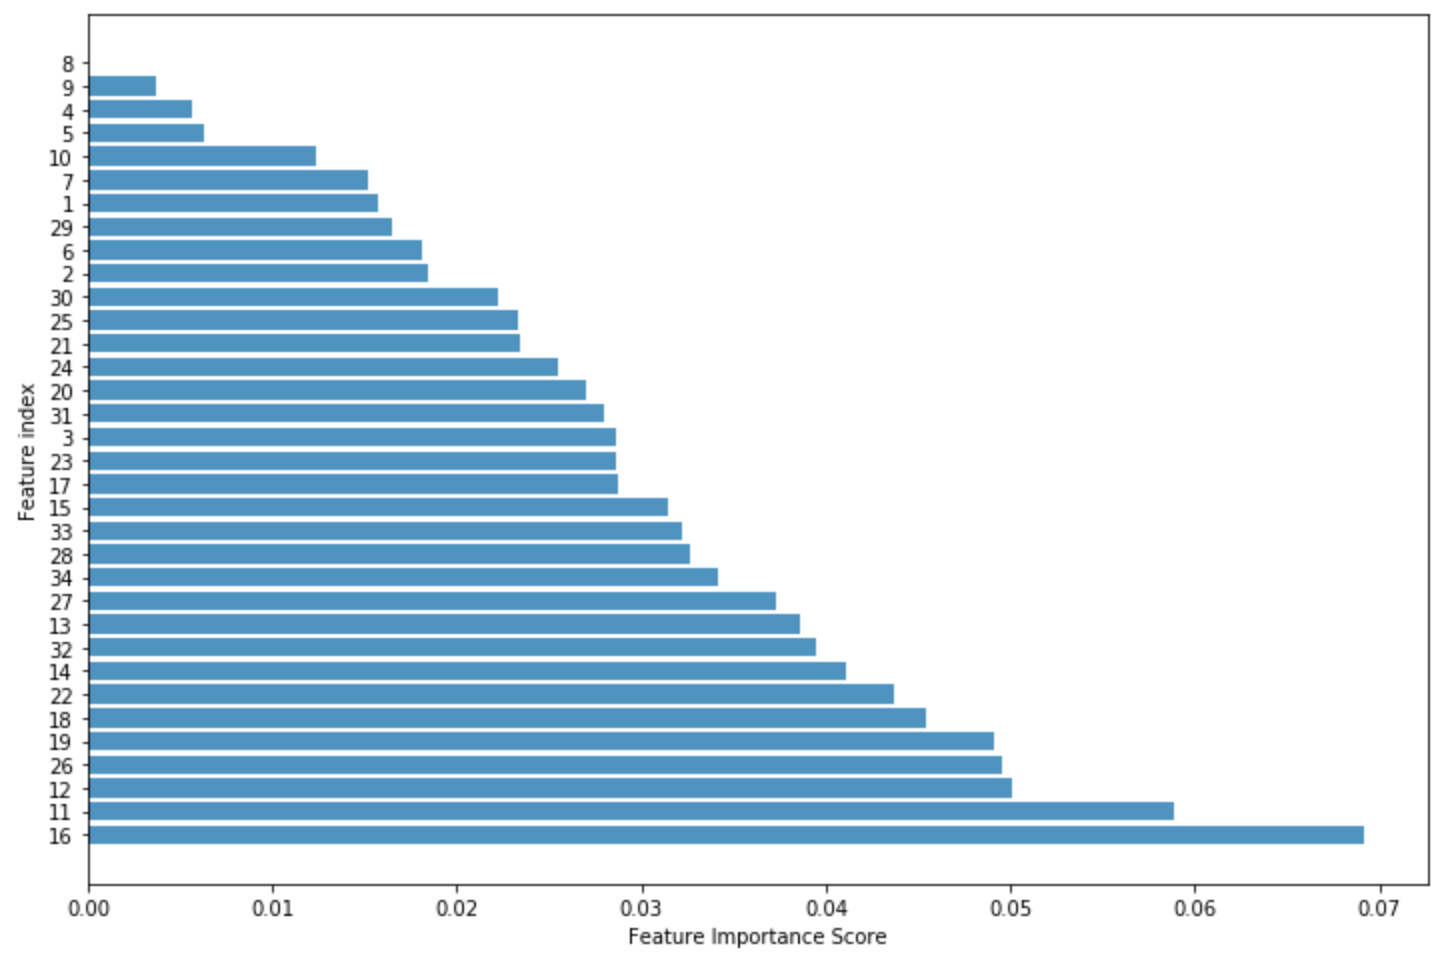
\includegraphics[width=\linewidth]{img/query_f_importance.png}
  \caption{Feature importance scores for the query recency sensitivity model.}
  \label{fig:fscores-queries}
\end{figure}
% plotted in queries.ipynb

We plot the first tree created in the model to gain insight into the decision process. The tree is shown in Figure \ref{fig:query_tree0}. We can see that the first decision is based on feature 10, but as the features are 0-indexed in the implementation, this is actually feature with index 11 from Table \ref{tb:features-query}, \texttt{LM\_Tweet\_2\_Day}. The next level is based on features with indices 1 and 2, \texttt{QuerySubmissions\_LastDay} and \texttt{QuerySubmissions\_LastWeek}. Arriving to the first leaf of the tree, the model concludes that if the probability of the language model based on bigrams from tweets from the past day is lower than a certain threshold, and the query was submitted less than 8 times in the past week, the resulting contribution to the overall score is 0.002, a very small value.

\begin{figure}
  \centering
  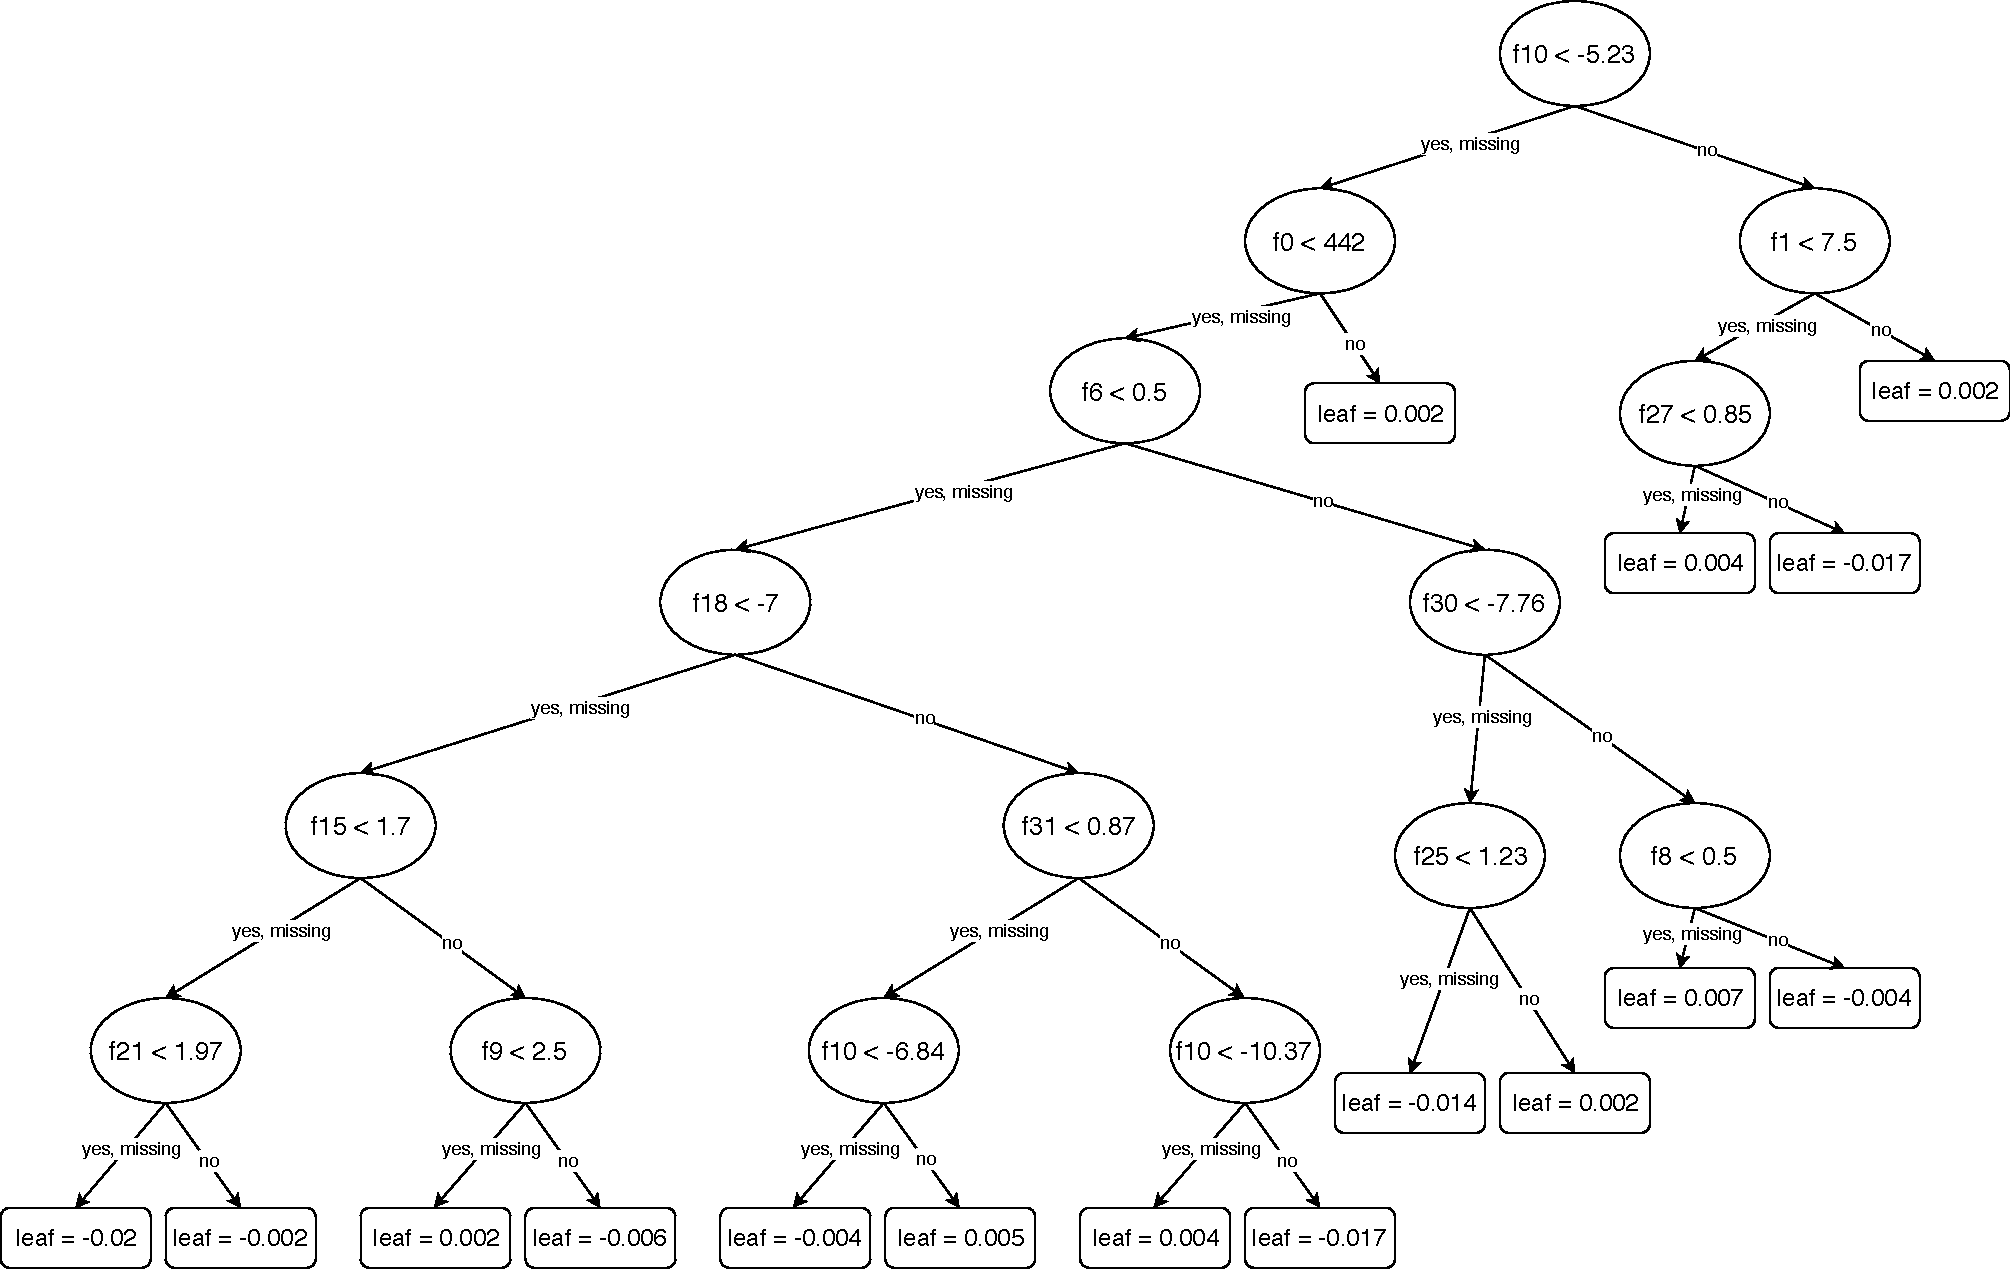
\includegraphics[width=\linewidth]{img/tree.pdf}
  \caption{First tree of the query recency sensitivity model.}
  \label{fig:query_tree0}
\end{figure}

\section{Evaluation}
For training the model, we split the input set into train and validation sets in the 70:30 ratio. We then proceed to grid search the hyper-parameters of the model using a 5-fold cross-validation. Listing~\ref{param-query} shows which hyper-parameters are tuned.

\begin{lstlisting}[language=json,caption=Hyper-parameter tuning for the query recency sensitivity model.,label=param-query]
'max_depth': [4, 6, 8, 10],	(best = 6)
'min_child_weight': [0, 1, 2],	(best = 0)
'gamma': [0.0, 0.1, 0.2, 0.3],	(best = 0.0)
'subsample': [0.6, 0.8, 1.0],	(best = 0.6)
'colsample_bytree': [0.6, 0.8, 1.0],	(best = 0.6)
'learning_rate': [0.01, 0.03, 0.1, 0.2, 0.3],	(best = 0.01)
'n_estimators': [100, 500, 1000, 5000]	(best = 500)
\end{lstlisting}

%  Best hyperparameters:
% {'colsample_bytree': 0.6, 'learning_rate': 0.01, 'min_child_weight': 0, 'n_estimators': 500, 'subsample': 0.6, 'max_depth': 6, 'gamma': 0.0}
% RMSE (train) 0.084499281335
% RMSE (test): 0.1077
% 1706.14706233

The hyper-parameters are explained in detail earlier in the thesis, in Section~\ref{sec:docparams}. We also set the model to stop learning if there are not any improvements after 50 rounds.

The training of the model took 28 hours on a machine with CentOS 7.5.1804, 16 GB of RAM, and 8 Intel(R) Xeon(R) CPU E5-2660 v3 @ 2.60GHz CPUs. The model was trained by minimizing the root mean squared error (RMSE) of the difference between the predicted query recency sensitivity score and the ground truth label (possible values: \texttt{0.0, 0.25, 0.75, 0.95}).

\begin{table}[h!]
\centering
\caption{Query recency sensitivity model evaluation.}
\label{tb:queryclass}
\begin{tabular}{@{}cc@{}}
\toprule
RMSE train & RMSE test \\ \midrule
0.0845  & 0.1077 \\ \bottomrule
\end{tabular}
\end{table}

The results on the train and test sets are shown in Table \ref{tb:queryclass}. Here, we report three queries with the highest predicted recency sensitivity score. The queries are taken from our web ranking ground truth collection, consisting of query-document pairs. The queries are:
\begin{enumerate}
	\item \textit{youtube}, submitted at \texttt{2017-08-20}. We explain this by looking at the snippets of the retrieved results. Most of the top ten results were less than a day old.
    \item \textit{daca news}, submitted at \texttt{2017-09-05}. This was a very hot topic in early September, and most retrieved results were news published on the same day.
    \item \textit{utah}, submitted at \texttt{2017-08-16}. There was a spike in this query's popularity due to wildfires in Utah.
\end{enumerate}

To gain additional insight into how our model is performing, we plot two different learning curves. The motivation for these learning curves is explained in detail earlier, in Section~\ref{sec:docparams}. The first learning curve, shown in Figure \ref{fig:query-curve1}, shows the model performance based on the number of training rounds. This graph can indicate if we can benefit from adding more training instances. In our case, we did not manually annotate data, so adding more instances should not be a problem. By looking at the validation error, we can see that the model's ability to generalize on unseen data plateaus at around 800 instances.

The second learning curve is shown in Figure \ref{fig:query-curve2}. Here, we examine the model's performance based on the number of training rounds. We notice that both the training and validation error reduce rapidly. Nevertheless, the validation error does not reduce significantly after 300 rounds, making it a valid cut-off candidate.

\begin{figure}[h]
\centering
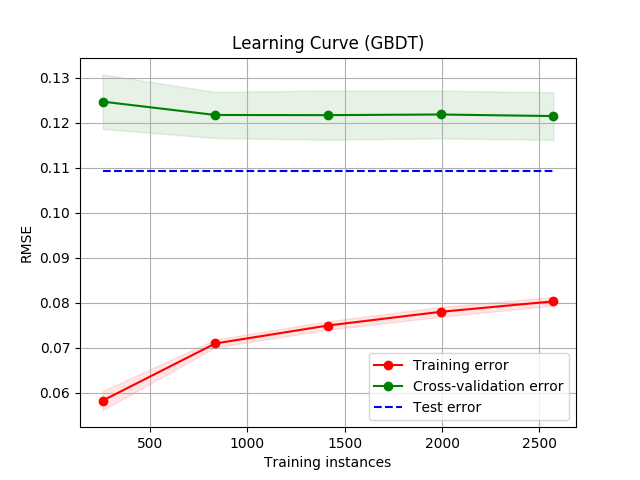
\includegraphics[width=0.8\linewidth]{img/query_learning_curve.png}
\caption{Learning curve of the query recency sensitivity model based on the number of training instances.}
\label{fig:query-curve1}
\end{figure}

\begin{figure}[h]
\centering
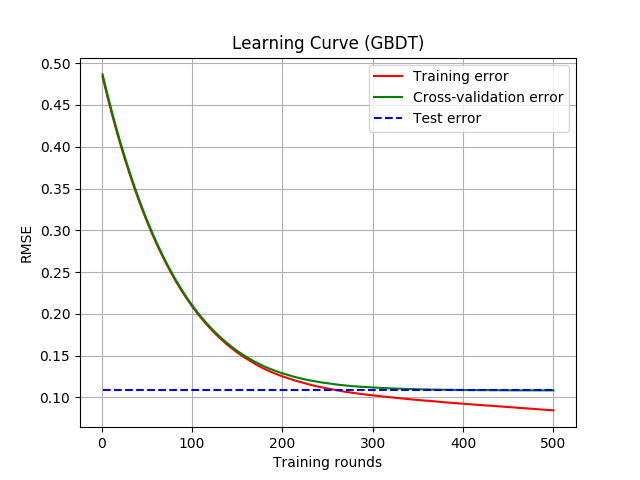
\includegraphics[width=0.8\linewidth]{img/query_learning_curve2.png}
\caption{Learning curve of the query recency sensitivity model based on the number of training rounds.}
\label{fig:query-curve2}
\end{figure}


\chapter{Incorporating Recency in Web Search}
\label{ch:webranking}

Currently, the commercial search engine ranks documents according to their relevance to the query. As mentioned earlier, in this work we are upgrading an existing commercial search engine prototype to support recency as well. To further improve the quality of the search engine, we introduce the recency component on the query and the document side. The rest of this chapter first outlines the architecture of the commercial search engine, then describes in detail how the two machine-learning models explained in Chapters \ref{ch:doc} and \ref{ch:query} are integrated.

\section{Search Engine Architecture}

The architecture of a search engine begins with crawling documents from the Web and ends with retrieving and ranking a subset of documents that best match a given search query. This can be done in multiple stages, and we identify the main stages as crawling, document selection, indexing, and ranking. Furthermore, the stages can be divided into two different groups: offline and online. An offline stage is query-independent and can be done in an offline manner, i.e., once in the beginning and later only when needed. On the other hand, online stages are query-dependent and are run any time a query is submitted. A high-level overview of ranking stages of the commercial search engine is shown in Figure \ref{fig:arch}.

The indexing and ranking stages are supported by Elasticsearch.\footnote{\url{https://www.elastic.co/products/elasticsearch}.} Described in \citep{gormley2015elasticsearch}, Elasticsearch is a distributed, scalable, real-time search and analytics engine. It is built on top of Apache Lucene,\footnote{\url{https://lucene.apache.org/core/}.} a search-engine library written in Java. Elasticsearch uses Lucene internally for indexing and searching, but extends the usability by exposing an easy-to-use RESTful API. The indexing and ranking stages are explained in more detail in their respective sections.

\begin{figure}
  \centering
  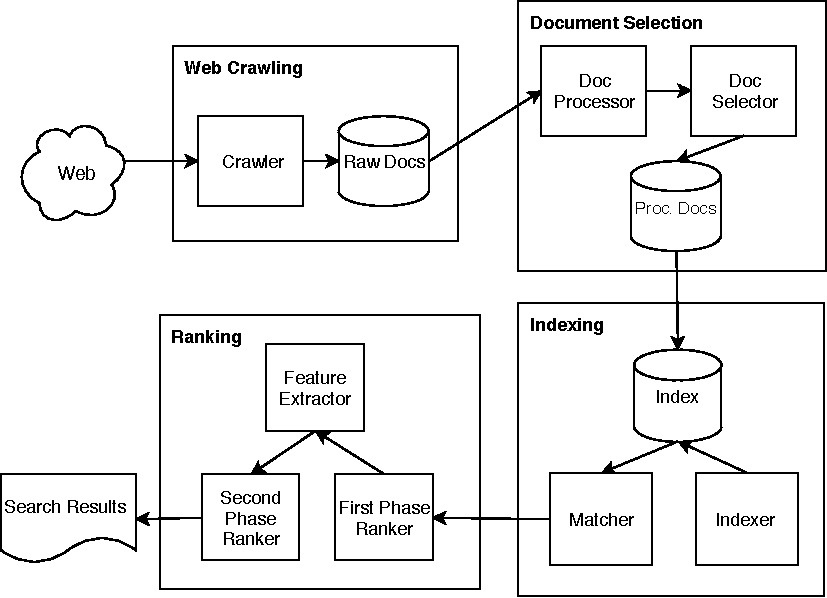
\includegraphics[width=\linewidth]{img/webranking.pdf}
  \caption{High-level architecture of the commercial search engine.}
  \label{fig:arch}
\end{figure}

\subsection{Web Crawling}
A crawler (or spider, robot, etc.) is a program that traverses the Web and downloads raw documents to a database. The two main tasks of a crawler are discovery and download of new pages and refreshing of the existing pages. The simplest approach is to start with a seed set of URLs, download the pages the URLs point to, then scan these pages for new links, add them to the queue of pages to be crawled, and repeat the process.

The crawler is an important component of a search engine, especially with regard to recency. For example, if there has been a breaking event and users search for it, if the crawler still has not crawled the relevant documents, they cannot be shown to the user. Therefore, a good crawler must download content fast enough so it does not become the bottleneck of the entire process.

\subsection{Document Selection}
The crawler can download a very large and diverse amount of content from the Web. However, not all of that content is useful. For example, we do not want to waste resources processing spam content. Therefore, the document selection stage filters out unnecessary documents, and stores the rest to be indexed. This stage consists of two modules: \texttt{Document Processor} and \texttt{Document Selector}. 

\texttt{Document Processor} is in charge of boilerplate removal and feature extraction. Boilerplate removal implies removing boilerplate parts from the Web page content (e.g., menus, footer, side bar) and unrelated parts (e.g., adverts, related articles). Consequently, we are left with a ``clean'' HTML, and we can extract features from the HTML and URL of the page, such as the number of tags and characters in the HTML, number of links, length of the link, etc.

\texttt{Document Selector} performs filtering of unwanted documents. It is a machine-learned regression model using Gradient Boosted Decision Trees (GBDT) to predict a document score. The features used are extracted from the HTML and the URL of the document. If the score of a document is below a certain threshold, it is discarded. Otherwise, the document is passed to the indexing stage. The scores are stored in a database, and the low-quality documents are removed periodically from the \texttt{Raw Docs} database.

\subsection{Indexing}
After a document is processed and stored in the \texttt{Processed Docs} database, it is sent to the indexing stage. Generally speaking, an index is a data structure that provides efficient retrieval for a given query. As mentioned earlier, this stage is handled by Elasticsearch and is run on an Elasticsearch cluster.

In Elasticsearch, documents are stored in an index as JSON objects which contain zero or more fields, or key-value pairs. In the \texttt{Document Selection} stage, \texttt{Document Processor} extracted features from the document content and its URL. These features are injected into the Elasticsearch index as key-value pairs in the document JSON.

An example of a simple keyword search query and a response from an index in Elasticsearch is shown in Listing \ref{es-search}. Additionally, Elasticsearch provides a Query DSL (Domain Specific Language) based on JSON to define queries, which is the way we query our indexes. An example of such query is shown in Listing \ref{es-search2}.

\begin{lstlisting}[language=json,firstnumber=1,caption=Example of a keyword search query and response in Elasticsearch., label=es-search]]
curl -XGET localhost:9200/books/_search?q=elasticsearch
{
  "took" : 2, "timed_out" : false,
  "_shards" : { "total" : 5, "successful" : 5, "failed" : 0 },
  "hits" : {
    "total" : 1, "max_score" : 0.076713204,
    "hits" : [ {
      "_index" : "books", "\_type" : "book", "\_id" : "1",
      "_score" : 0.076713204, "_source" : {
        "title" : "Elasticsearch - The definitive guide",
        "authors" : [ "Clinton Gormley", "Zachary Tong" ],
        "started" : "2013-02-04", "pages" : 230
      }
    } ]
  }
}
\end{lstlisting}

\begin{lstlisting}[language=json,firstnumber=1,caption=Example of a search query specified in DSL in Elasticsearch., label=es-search2]]
curl -XGET 'localhost:9200/books/book/\_search' -d '{
  "query": {
    "filtered" : {
      "query" : {
        "match": {
          "text" : {
            "query" : "To Be Or Not To Be",
            "cutoff_frequency" : 0.01
          }
        }
      },
      "filter" : {
        "range": {
          "price": {
            "gte": 20.0
            "lte": 50.0
   ...
  }
}'
\end{lstlisting}

The underlying data structure Elasticsearch uses for its index is the inverted index, designed to allow fast full-text searches. An inverted index consists of a list of all the unique words that appear in any document, and for each word, a list of the documents in which it appears. For example, if we have two documents $D_1$ = \textit{Madrid is the capital of Spain} and $D_2$ = \textit{Barcelona is the capital of Catalonia}. To create an inverted index, we first split the contents of each document into separate words, or tokens, normalize them, create a sorted list of all the unique tokens, and then list in which document each term appears. An example of such inverted index is shown in Table \ref{tb:inv-index}. If we want to search for \textit{capital spain}, we just need to find the documents in which each tokens appears, in this case the count is 2 for $D_1$, and 1 for $D_2$, so document $D_1$ seems more relevant for this query.

\begin{table}[]
\centering
\caption{A simple example of an inverted index.}
\label{tb:inv-index}
\begin{tabular}{@{}ccc@{}}
\toprule
Token & $D_1$ & $D_2$ \\ \midrule
barcelona & - & x \\
capital & x & x \\
catalonia & - & x \\
is & x & x \\
madrid & x & - \\
of & x & x \\
spain & x & - \\
the & x & x \\ \bottomrule
\end{tabular}
\end{table}

The indexing phase is finished when the document has been preprocessed, and the features have been extracted and stored as fields in the JSON object representing it.

\subsection{Ranking}
After the document has been indexed, once a user query is submitted, the \texttt{Matcher} matches the documents for the query. The matching is done by performing a logical conjunction (operator \texttt{AND}) between all of the terms from the query and the content of the document. Once we identify matching documents for a query, we can score them and rank them.

The ranking stage takes care of computing the relevance scores of the matching documents for the query and ranking them. Since there could be potentially millions of matching documents, computing all of the scores can be quite expensive. Therefore, we resort to a two-stage ranking architecture, where the first phase is essentially a cheap, but effective filter. The idea is to use query-independent features in the first phase ranking, because they can be precomputed in an offline manner and accessed by a simple lookup at query processing time. The first phase ranking function assigns scores to all of the matching documents $N$, and we only take the top $M$ ($M << N$) for the next stage. Since we now have a substantially smaller subset of the initial matching documents, we can extract more sophisticated and computationally expensive features. Finally, the second phase ranking function produces the ranking of the documents that are shown to the user.

We use and customize the Elasticsearch Learning to Rank plugin\footnote{\url{https://github.com/o19s/elasticsearch-learning-to-rank}.} for storing features, training datasets, models, and ranking the documents. We use the RankLib library\footnote{\url{https://sourceforge.net/p/lemur/wiki/RankLib/}.} to train the ranking models. Each model is described in its respective section as follows.

\subsubsection{First Phase Ranking}
In the first phase, we extract a combination of query-dependent and query-independent features. As described by \citet{cambazoglu2010early}, the first phase is used for selecting a small subset of potentially relevant documents from the entire collection. The typical features in this stage are:
\begin{itemize}
	\item \texttt{DocScore:} The score of the document produced in the Document Selection stage by the \texttt{Document Selector}. This score is also used as an indicator if we should index a document or discard it;
    \item \texttt{BM25(query, content):} The score of the $BM25$ function between the query and the content of the document.
\end{itemize}

The $\text{BM}25$ function \citep{robertson1996okapi} is a ranking function that can be computed automatically, without needing any relevance information. Given a query $Q$ containing keywords $q_1, ..., q_n$, the BM25 score of a document $D$ is:
\[ \text{BM}25(Q, D)=\sum _{i=1}^{n}{\text{IDF}}(q_{i})\cdot {\frac {f(q_{i},D)\cdot (k_{1}+1)}{f(q_{i},D)+k_{1}\cdot \left(1-b+b\cdot {\frac {|D|}{\text{avgdl}}}\right)}} \]

\noindent Here, $f(q_i, D)$ is $q_i$'s term frequency in the document $D$, $|D|$ is the length of the document $D$ in words, and $avgdl$ is the average document length in the text collection from which documents are drawn. Moreover, $k_1$ and $b$ are free parameters, and their default value in Elasticsearch is $k_1 = 1.2$ and $b = 0.75$. $\text{IDF}(q_i)$ is the inverse document frequency weight of the query term $q_i$. It is usually computed as:
\[ \text{IDF}(q_i) = \log \frac{N - n(q_i) + 0.5}{n(q_i) + 0.5} \]

\noindent Here, $N$ is the total number of documents in the collection, and $n(q_i)$ is the number of documents containing $q_i$.

Finally, we rank all the matching documents according to their first phase score, and get the top $M$ results, where $M << N$.

\subsubsection{Second Phase Ranking}
Contrary to the scoring function in the first phase, the second phase function is more complex. Since we only have a subset of documents to rank, we can afford extracting more computationally heavy features and training a more sophisticated model. The ranking produced by this model is the final ranking shown to the user. The model uses hundreds of features. Examples of different feature types are listed as follows:

\begin{itemize}
	\item \texttt{Query string.}\ Number of words, boolean features, etc.
    \item \texttt{URL string.}\ URL length, slash count, etc.
    \item \texttt{Document content.}\ Number of pictures, different tags, etc.
    \item \texttt{Content classification.}\ Output of classifiers of document content for spam, malware, adult content, etc.
    \item \texttt{Content-query relevance.} $\text{BM}25$ scores for query-title, query-URL, query-body, etc.
    \item \texttt{Content-query similarity.}\ Jaccard similarity or edit distance between the query and title, URL, etc.
    \item \texttt{Web graph.}\ PageRank, TrustRank, indegree, outdegree, etc.
    \item \texttt{Wikipedia.}\ Wikipedia page view count, references from Wikipedia, etc.
    \item \texttt{Traffic data.}\ The Alexa Traffic rank.\footnote{\url{https://www.alexa.com/siteinfo}.}
    \item \texttt{Document score.}\ Computed by the \texttt{Document Selector} model, trained using query-independent features.
    \item \texttt{First phase score.}\ Computed according to the ranking model in the first phase.
\end{itemize}

The offline features (query-independent) are computed and injected into the Elasticsearch index as document fields. The online features (query-dependent) are computed at query processing time using our customized Elasticsearch ranking plugin.

In this work, we introduce a type of features called \texttt{Recency features}, consisting of predicted document age and predicted query recency sensitivity. The document age feature is computed offline and injected into the ES index, whereas the query recency sensitivity feature should be computed at query processing time.

\section{Offline Experiments and Results}
In this section, we explain how we integrate the models explained in Chapters \ref{ch:doc} and \ref{ch:query} with the existing multi-stage ranking architecture. Our goal is to investigate whether the addition of recency features improves the overall ranking.

Both recency models, document age prediction and query recency sensitivity, are developed in a Hadoop cluster, and the extracted features and predictions are stored in HDFS. Apache Hadoop\footnote{\url{http://hadoop.apache.org/}.} is a free, open source, Java-based programming framework for distributed processing of large data sets across clusters of computers. Hadoop provides its own file system, called Hadoop Distributed File System (HDFS). Moreover, Hadoop handles job scheduling and cluster resource management, as well as parallel processing of large data sets. Both models run in Spark,\footnote{\url{http://spark.apache.org/}.} a fast and general compute engine for Hadoop data. The query recency sensitivity model is written in Python, using PySpark,\footnote{\url{https://spark.apache.org/docs/0.9.0/python-programming-guide.html}} the Spark Python API. The document age prediction model is written in Scala, which is supported natively in Spark.

\subsection{Model Integration}
Figure \ref{fig:docmodel} shows the integration of the document age prediction model into the existing ranking architecture. As described in Chapter \ref{ch:doc}, the ground truth is obtained by querying Memgator, an external web service. The script to build the ground truth, and the script to extract features are both written in Scala, run in Spark on the Hadoop cluster, and save the output data to HDFS. 

The document age model training module is written in Python to make use of XGBoost's Python API in scikit-learn.\footnote{\url{http://scikit-learn.org/stable/}.} We also run it on the Hadoop cluster, and save the predicted values to HDFS. Next, the Elasticsearch Feature Injector runs in Spark to read the predicted document last update time and inject it to Elasticsearch's index. Finally, we extend the Elasticsearch ranking plugin to calculate the document age as $currentTime - documentLastUpdateTime$ when queried (during the ranking models' training time).

\begin{figure}
  \centering
  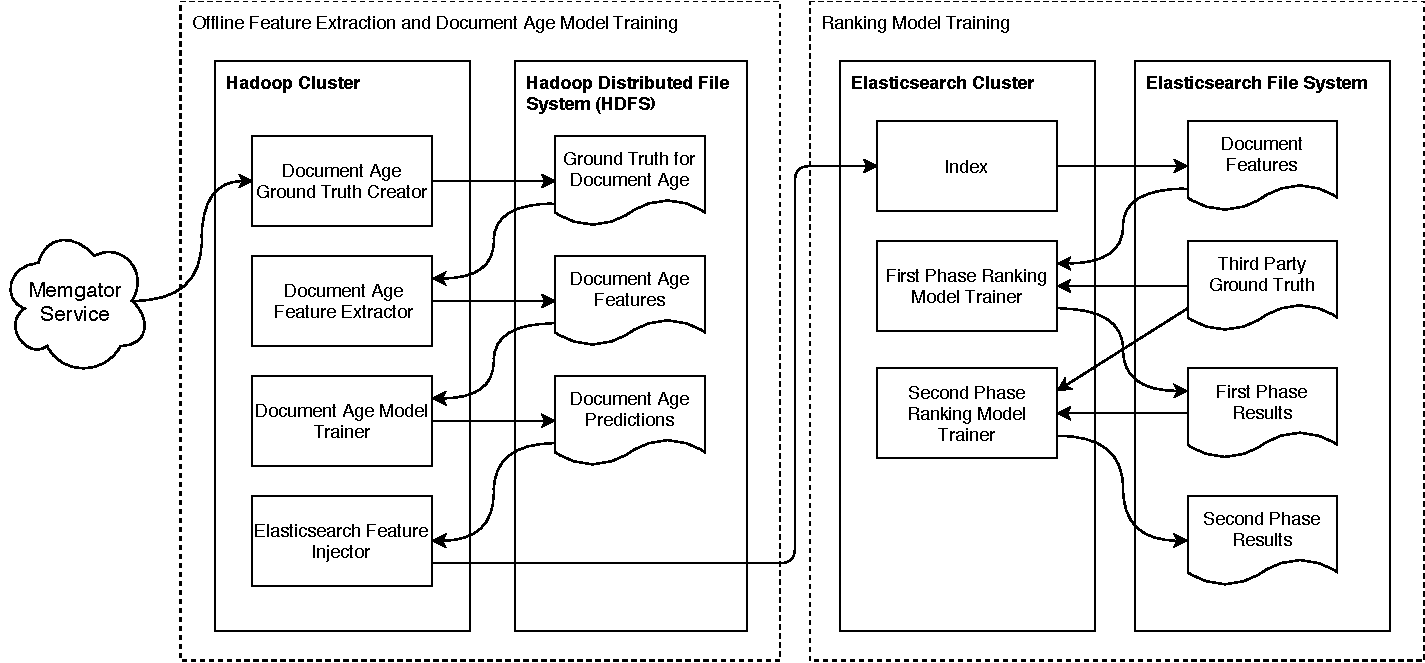
\includegraphics[width=\linewidth]{img/docmodel.pdf}
  \caption{Integration of the document age prediction model into the existing ranking pipeline.}
  \label{fig:docmodel}
\end{figure}

Figure \ref{fig:querymodel} shows the integration of the query recency sensitivity model into the existing ranking architecture. This model is described in detail in Chapter \ref{ch:query}. It is more complicated than the previous model in terms of external calls, because the corpora needed to build the language models is obtained from external sources such as Twitter and the query log. The ground truth is created by a PySpark script run in Spark on the Hadoop cluster that automatically labels queries according to the retrieved web snippets, and stores the output to HDFS.

The module that mines the Twitter corpus is a combination of Bash scripts (to retrieve the tweets using \texttt{twarc} and to extract the data) and PySpark (to filter and process the data, and save it to HDFS). The module that mines the query log corpus is a PySpark script that runs in Spark on the Hadoop cluster and saves the output to HDFS. The module that creates language models from both types of corpora is a Bash script which saves the resulting language models to HDFS. Next, the feature extractor is a combination of Bash scripts (to download the language models locally and to predict the language model feature type values) and PySpark (to extract the other feature type values).

Next, we need to inject the predictions of the query recency sensitivity model to the existing ranking pipeline. Since these predictions are related to the query itself, not the document, they cannot just be injected to the document index. Therefore, we inject them to our third party ground truth file used for training the ranking models. This is done by a Bash script that runs on the Elasticsearch cluster. The ground truth file consists of query-document pairs, so we simply append the query recency sensitivity score to each query-document pair. Finally, the recency sensitivity score is used as a feature in both the first- and second-phase ranking models.

\begin{figure}
  \centering
  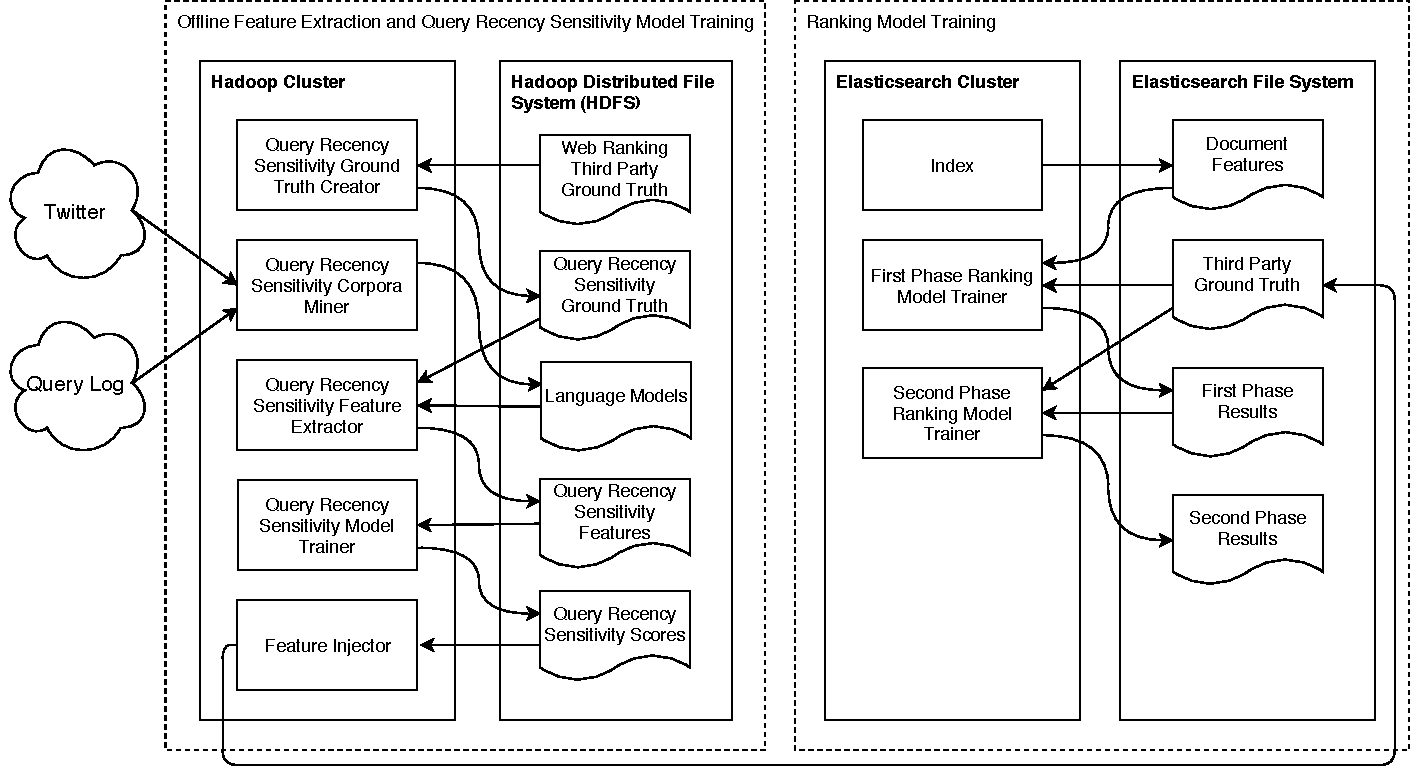
\includegraphics[width=\linewidth]{img/querymodel.pdf}
  \caption{Integration of the query recency sensitivity model into the existing ranking pipeline.}
  \label{fig:querymodel}
\end{figure}

\subsection{Recency Ranking Results}
The initial research question we asked ourselves is whether introducing recency features boosts the overall ranking performance. Since we are interested in the end result, or the quality of the search results shown to the user, we report the performance of the second-phase ranking model (which, in turn, also depends on the first-phase model, since its output is used as a feature).

Table \ref{tb:res} shows the evaluation of different ranking models. The evaluation metric used is NDCG@10 with respect to a third party search engine. The first model, denoted as F, is the model without any recency features. When adding just the document age feature (model F+1), we observe an increase in NDCG@10 of 0.35\%. This means that the model is now able to capture recency on the document side, but still not on the query side. In other words, it might learn to favour more recent documents in general, irrespective of the query. Furthermore, we add the query recency sensitivity score (model F+2), an observe an total increase in NDCG@10 of 0.48\%. Now, the model is able to learn to what extent to favour recent documents depending on the query. For example, if the query recency sensitivity score is low, there is no need to boost more recent documents. On the other hand, if the query recency sensitivity score is high, the ranking should be different than the one so far, without taking recency into account. In other words, more recent documents should be favoured.

Overall, we have introduced only two new features to the existing hundreds of features, and gained 0.48\% improvement in NDCG@10. Moreover, we evaluated the feature importances, shown in Table \ref{tb:f-imp-doc}. We can see that the model picks both features pretty early, as indicated by the rank of the tree they first appeared in. Therefore, the features are significant to the model's increase in performance.

\begin{table}[]
\centering
\caption{Evaluation of the recency feature importances in the second-phase ranking model.}
\label{tb:f-imp-doc}
\begin{tabular}{@{}ccccc@{}}
\toprule
Model & Feature name & Normalized feature rank & First appeared tree \\ \midrule
F+1 & documentAge & 0.72 & 541 (out of 2460) \\
F+2 & documentAge & 0.72 & 541 (out of 2937) \\
F+2 & queryRecencySensitivity & 0.73 & 660 (out of 2937) \\ \bottomrule
\end{tabular}
\end{table}

\begin{table}[]
\centering
\caption{Evaluation of the second-phase ranking model. Model F does not contain recency features, model F+1 contains the document age feature, and model F+2 contains both the document age feature and the query recency sensitivity score.}
\label{tb:res}
\begin{tabular}{@{}ccc@{}}
\toprule
Model & \multicolumn{1}{l}{Number of trees} & Improvement of NDCG@10 \\ \midrule
F & 1657 & - \\
F+1 & 2460 & 0.35\% \\
F+2 & 2937 & \textbf{0.48\%} \\ \bottomrule
\end{tabular}
\end{table}

\section{Online Integration and Future Work}
The previous section describes how we introduce the two recency features to the existing ranking models in an offline fashion. In other words, in that setup we are only training and evaluating the models. In an online, production setting, we want to be able to calculate these features on the fly. More specifically, when a user submits a query to the search engine, the document age model and the query recency sensitivity model must output a prediction.

Since the document age prediction model is not query-dependent, the online prediction involves calling the function in our Elasticsearch ranking plugin to calculate the document age with respect to the query submission time and the already injected document last update time, which is already supported.

However, for the online prediction of the query recency sensitivity model, we should already have the language models constructed and ready to use. This means we must already have the Twitter and query log corpora in place. As a reminder, we build language models based on the last day, week, and last two weeks (in case of tweets) or last month (in case of the query log). So, one challenge is to keep the language models fresh by updating the corpora they need daily. Another challenge, which has not been solved at to the time of writing, is to calculate query-dependent features in Elasticsearch which involve a call to an external store where the features would be located. This is a limitation of the ranking plugin we are using. Nevertheless, we are certain this feature will be supported soon, and the integration of it remains as future work. An example of an end-to-end online pipeline is shown in Figure \ref{fig:online}.

\begin{figure}
  \centering
  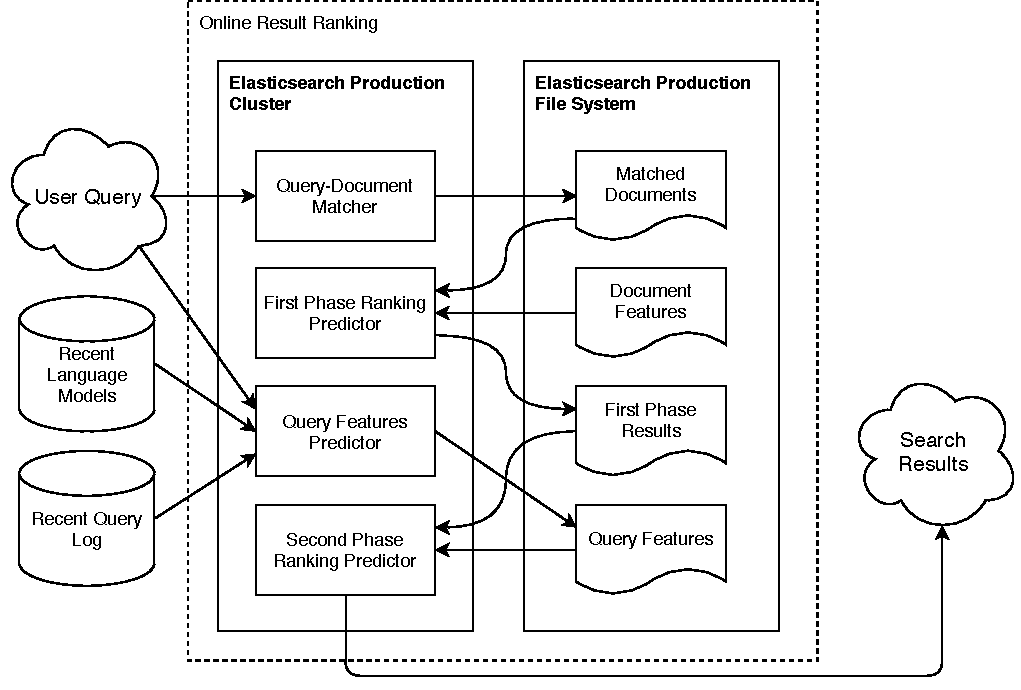
\includegraphics[width=\linewidth]{img/online.pdf}
  \caption{End-to-end pipeline for online result ranking.}
  \label{fig:online}
\end{figure}

\chapter{Conclusion}
\label{ch:conclusion}

Combining relevance and recency in Web search is an open problem. There are numerous approaches to this ranking problem, and existing solutions mostly focus on only one type of queries or documents. In this work, we introduce recency ranking for queries and documents on the Web in general, while preserving the existing relevance ranking.

We presented a novel combination of machine-learned models to predict recency, both on the query and document side. We propose a query recency sensitivity classifier to determine the need for recent documents, and a document age prediction model to determine how recent a document is.

We automatically labeled both ground truth datasets to avoid costly and time-consuming human annotation. We extracted features from several different sources. We recognized the challenges in keeping the feature values up to date and provided a solution on how to implement this in production. We trained two Gradient Boosted Regression Trees (GBRT) models and integrated them as features in an existing multi-stage ranking architecture.

Having added only two recency features, we managed to improve the NDCG@10 of our ranking model by 0.5\%. We consider this a very good improvement, given that the model is already rich in strong features. Moreover, we did not introduce significant increase in scoring time. Finally, the introduced features are not exact, but predicted, which means they are open to further improvement.

Our future work consists of improving the query recency sensitivity classifier and the document age prediction model. For the query classifier, introducing language models built from other sources such as news articles might be beneficial. For the document classifier, we are currently extracting only content-based features, whereas we could also make use of, for example, link-based features.


\bibliography{literatura}
% \bibliographystyle{fer}
\bibliographystyle{plainnat}

\begin{abstract}
Given the increase in the amount of accessible information on the Web, more attention has been drawn to information retrieval systems such as search engines. In web search, recency ranking refers to ranking documents by their relevance to the query, but also taking freshness into account. In this thesis, we propose two models for recency ranking. The first one is the query recency sensitivity model, and the second is a model to predict the publication time of documents. We extract temporal features from several sources and automatically construct ground truth datasets for both models. Furthermore, we integrate the models into an existing commercial search engine with a multi-stage ranking architecture. Our experiments demonstrate an improvement in the effectiveness of the commercial search engine.

\keywords{recency ranking, web search, search engine, machine learning, gradient boosted decision trees, information retrieval, big data}
\end{abstract}

\newpage

% TODO: Navedite naslov na hrvatskom jeziku.
\hrtitle{Modeli rangiranja po svježini za pretraživanje weba}
\begin{sazetak}
Porastom raspoloživih količina dostupnih informacija na Webu, povećalo se zanimanje za sustavima koji dohvaćaju informacije, poput sustava za pretraživanje. Pri pretraživanju weba, rangiranje po svježini odnosi se na rangiranje dokumenata s obzirom na relevantnost na upit, a pritom uključujući i svježinu rezultata. U okviru diplomskog rada prezentiramo dva modela za rangiranje po svježini. Prvi model predviđa osjetljivost upita na svježinu rezultata, a drugi predviđa vrijeme objavljivanja dokumenata. Gradimo vremenske značajke na temelju više izvora i automatski gradimo skup podataka za vrednovanje oba modela. Nadalje, integriramo modele u postojeći komercijalni pretraživač Weba koji se sastoji od višefazne arhitekture za rangiranje. Naši eksperimenti ukazuju na poboljšanje korisnosti komercijalnog pretraživača Weba.

\kljucnerijeci{pretraživanje po svježini, pretraživanje Weba, tražilica, strojno učenje, stabla odluke potpomognuta gradijentom, dohvat informacija, veliki skupovi podataka}
\end{sazetak}


\end{document}
